\section{Three-level system}\label{sec:pw3l}

A two-level system is the simplest non-trivial quantum system and,
as seen in Sec.~\ref{sec:absorption+pw},
it is sufficient to illustrate
models of quantum time of arrival,
such as those based on complex potentials,
as well as relational models.
Therein, numerical examples have been shown, where the two approaches
---discrete Page--Wootters and the ``non Hermitian'' detector models---
lead to
compatible predictions.

A three-level atom (or a three-level quantum system in general) appears
naturally
as
the next computational step;
but far from being merely another excercise
---just at a slightly higher level of complexity
but otherwise showing, essentially, the same physics---
it is in fact the \emph{minimal} system \emph{required}
to realize a broad
phenomenology that includes the
\term{Stimulated Raman adiabatic passage}
---STIRAP \parencite{Ruschhaupt_AtomDiode, NonHermitianShortcutSTIRAP, OptimizedTransferSTIRAP}
and the
\term{Electromagnetically induced transparency}
---EIT \parencite{EIT_Review}.

Also, it wil be shown that a three-level atom can model
a more robust and realistic
detector for time-of-arrival measurement, compared to the one implemented
with a two-level atom (as introduced in Sec.~\ref{sec:hist:detect}).
The atom can be ``driven'' by a laser
from the ground state $\ket{0}$ into the excited state $\ket{2}$,
then decay into a metastable state $\ket{1}$ at an intermediate energy
(see the above references, although they might use a slightly different notation).
This prevents the atom from decaying again and altering the ``arrival'' detection.

As usual, we're going to set $\hbar = 1$ in the following numerical computation,
based, once again, on the
\emph{NumPy} framework \parencite{comp:numpy},
within a
\term{Jupyter notebook} \parencite{comp:jupyter}.
Details can be consulted in the Appendix~\ref{detector-model-3-level-system}.
Full source code is available from the repository at ref. \cite{OwnJupyterRepo}.

%% {Figures}

% Probabilities

\begin{figure}[h]
  \begin{subfigure}[b]{\textwidth}
    \centering
    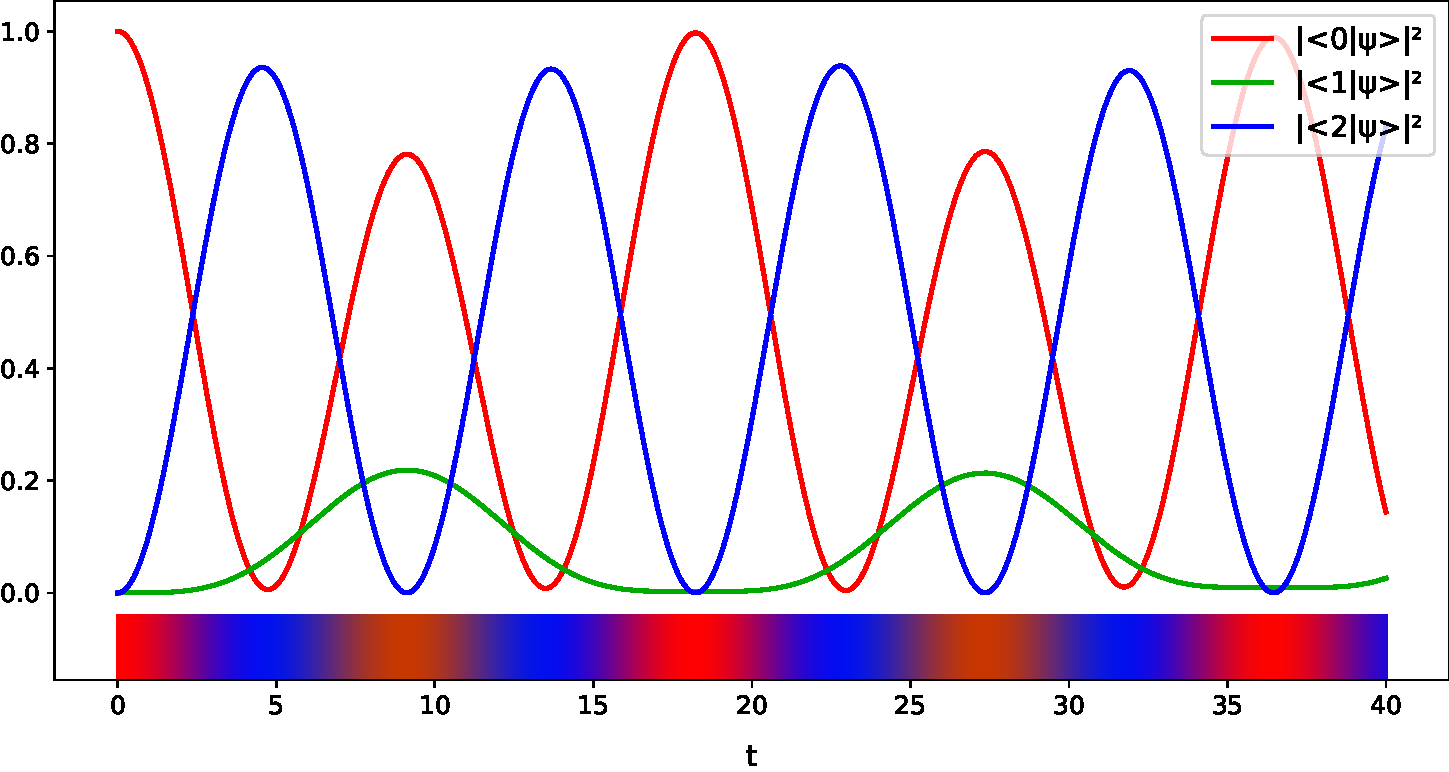
\includegraphics[width=.8\textwidth]{img/3ldetect/hermitian3lines.pdf}
    \subcaption{Foo.}%\label{fig:aabsorbed-qubit-components_pwlattice:re0}
  \end{subfigure}
  \par\bigskip
  \par\bigskip
  \begin{subfigure}[b]{\textwidth}
    \centering
    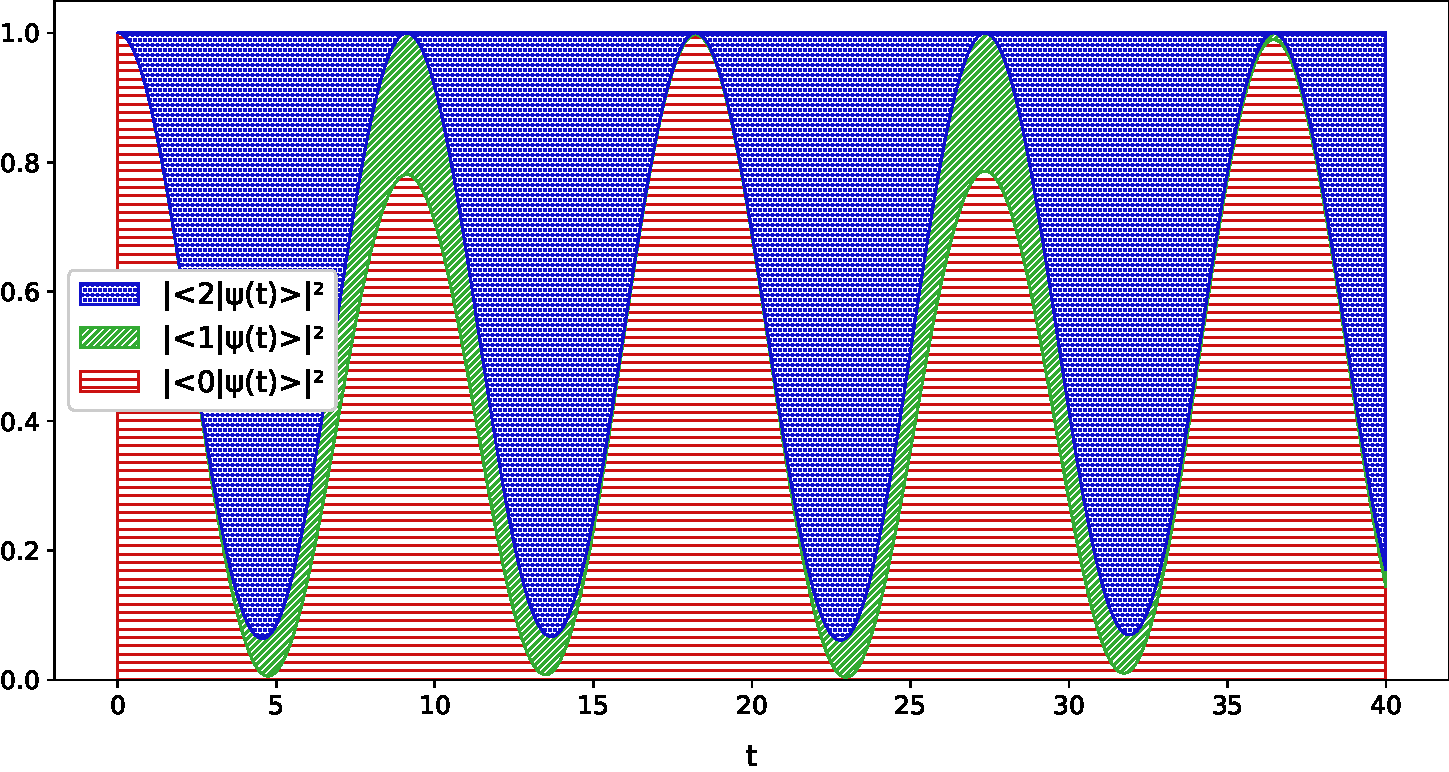
\includegraphics[width=.8\textwidth]{img/3ldetect/hermitian3color.pdf}
    \subcaption{Bar.}%\label{fig:aabsorbed-qubit-components_pwlattice:im1}
  \end{subfigure}
  \par\bigskip
  \par\bigskip
  \caption{
    Blah blah blah.
  }
  %\label{fig:aabsorbed-qubit-components_pwlattice}
\end{figure}

% \ContinuedFloat example

% \begin{figure}[hb!]
%   \centering
%   \begin{subfigure}{\textwidth}
%       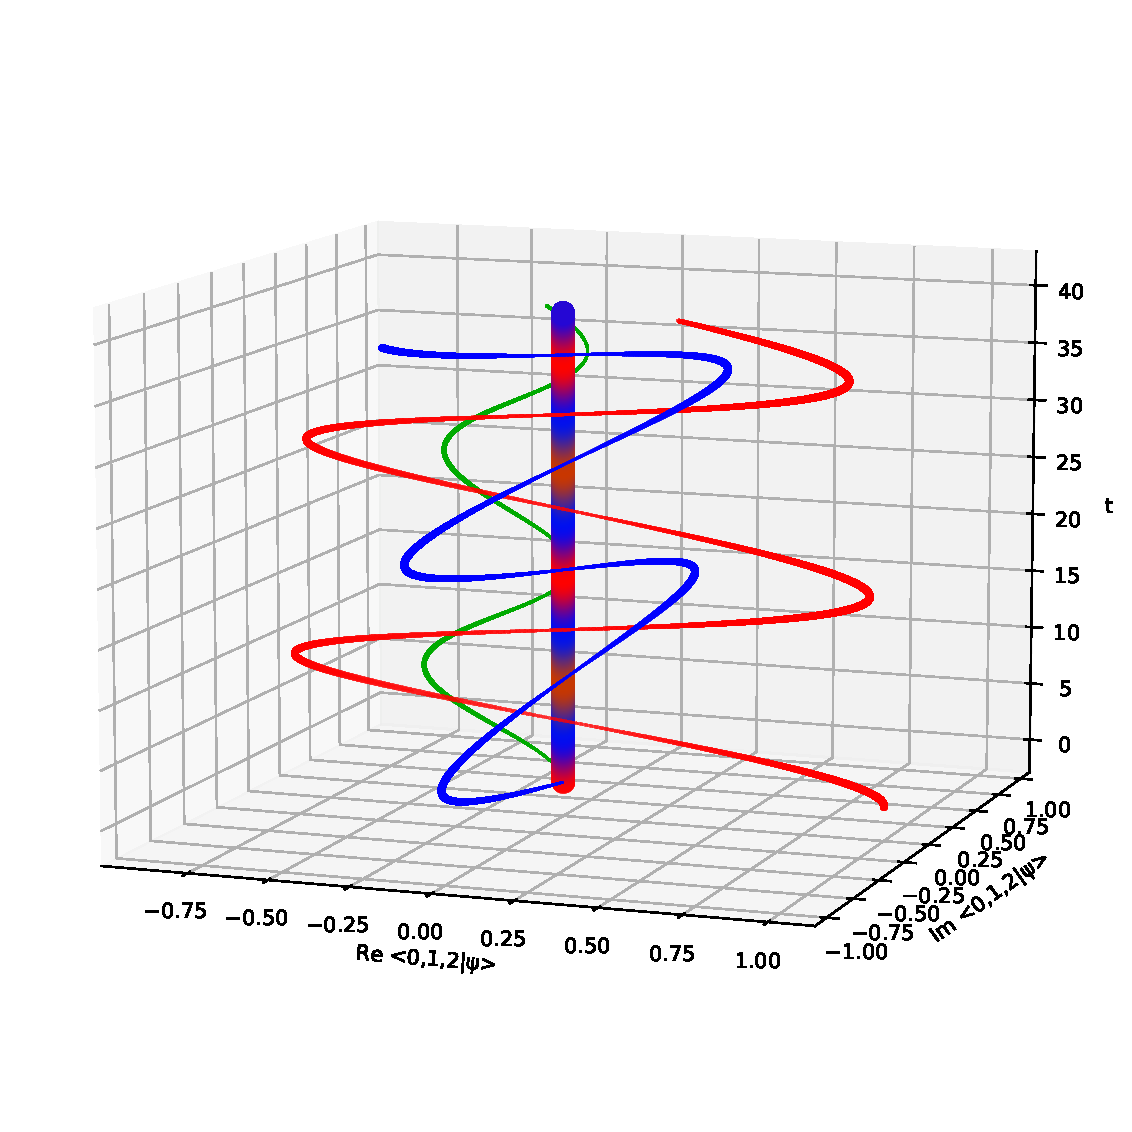
\includegraphics[width=\textwidth]{img/3ldetect/hermitianSpaceTime_side.pdf}
%       \subcaption{Foo.}
%       %\label{fig:arm1}
%   \end{subfigure}
%   \caption{Foobar.}
% \end{figure}%
% \begin{figure}[ht]\ContinuedFloat
%   \centering
%   \begin{subfigure}{\textwidth}
%       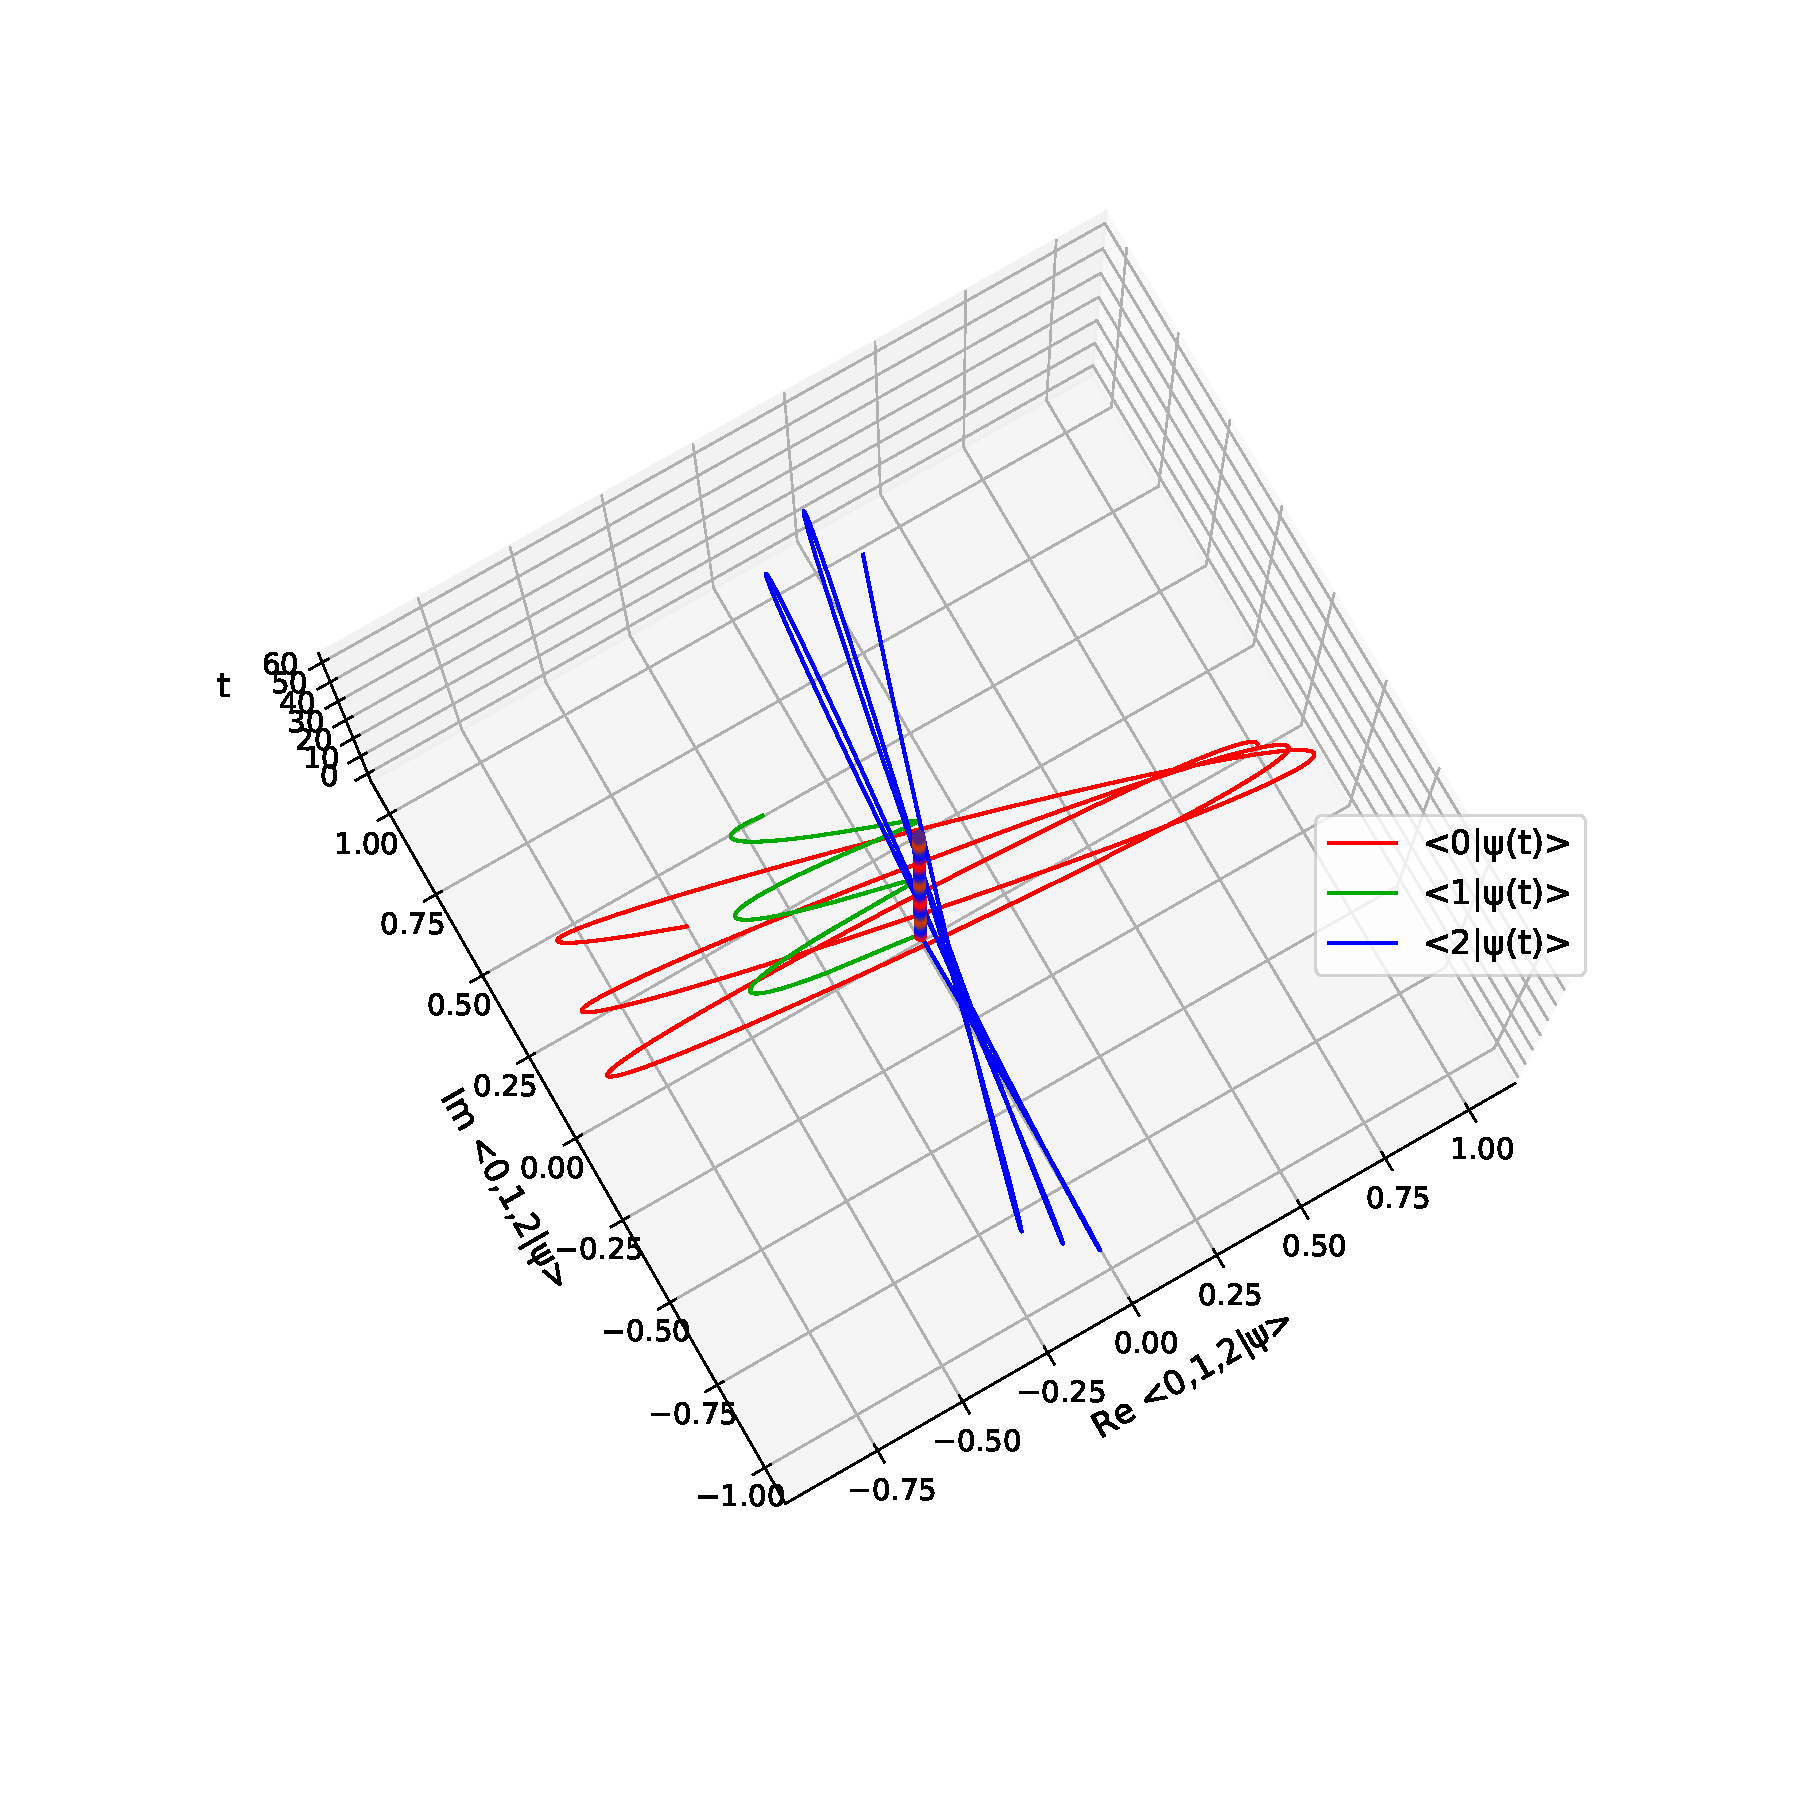
\includegraphics[width=\textwidth]{img/3ldetect/hermitianSpaceTime_top.pdf}
%       \subcaption{Bar.}
%       %\label{fig:arm3}
%   \end{subfigure}
%   \caption{Foobar (cont.)}
% \end{figure}

% "3D" evolution

\begin{figure}[h]
  \begin{subfigure}[b]{\textwidth}
    \centering
    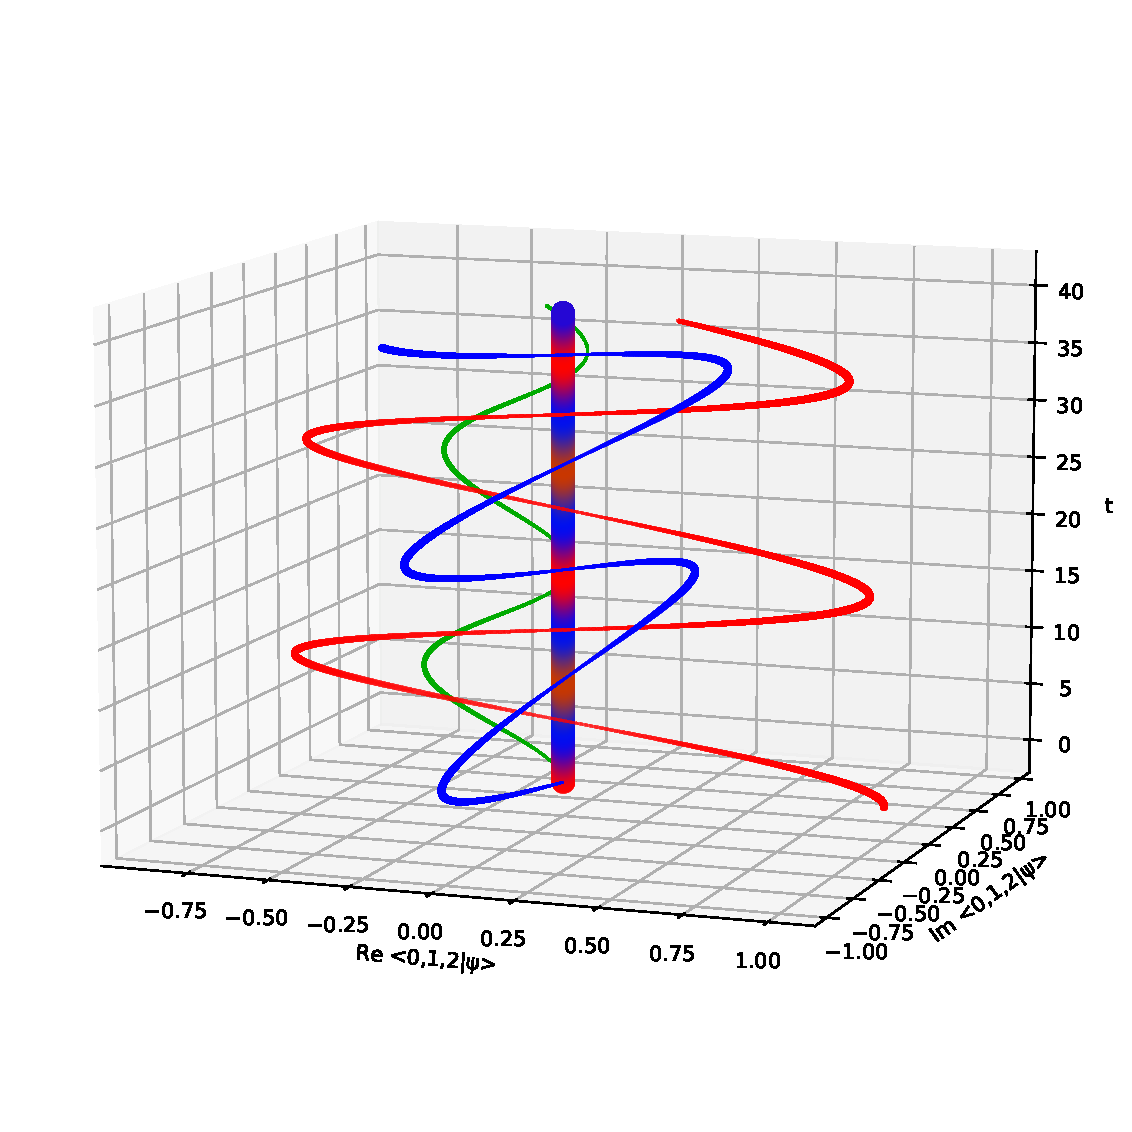
\includegraphics[height=0.45\textheight,clip,trim=80 180 40 140]{img/3ldetect/hermitianSpaceTime_side.pdf}
    \caption{Foo.}
  \end{subfigure}
  \par\bigskip
  \begin{subfigure}[b]{\textwidth}
    \centering
    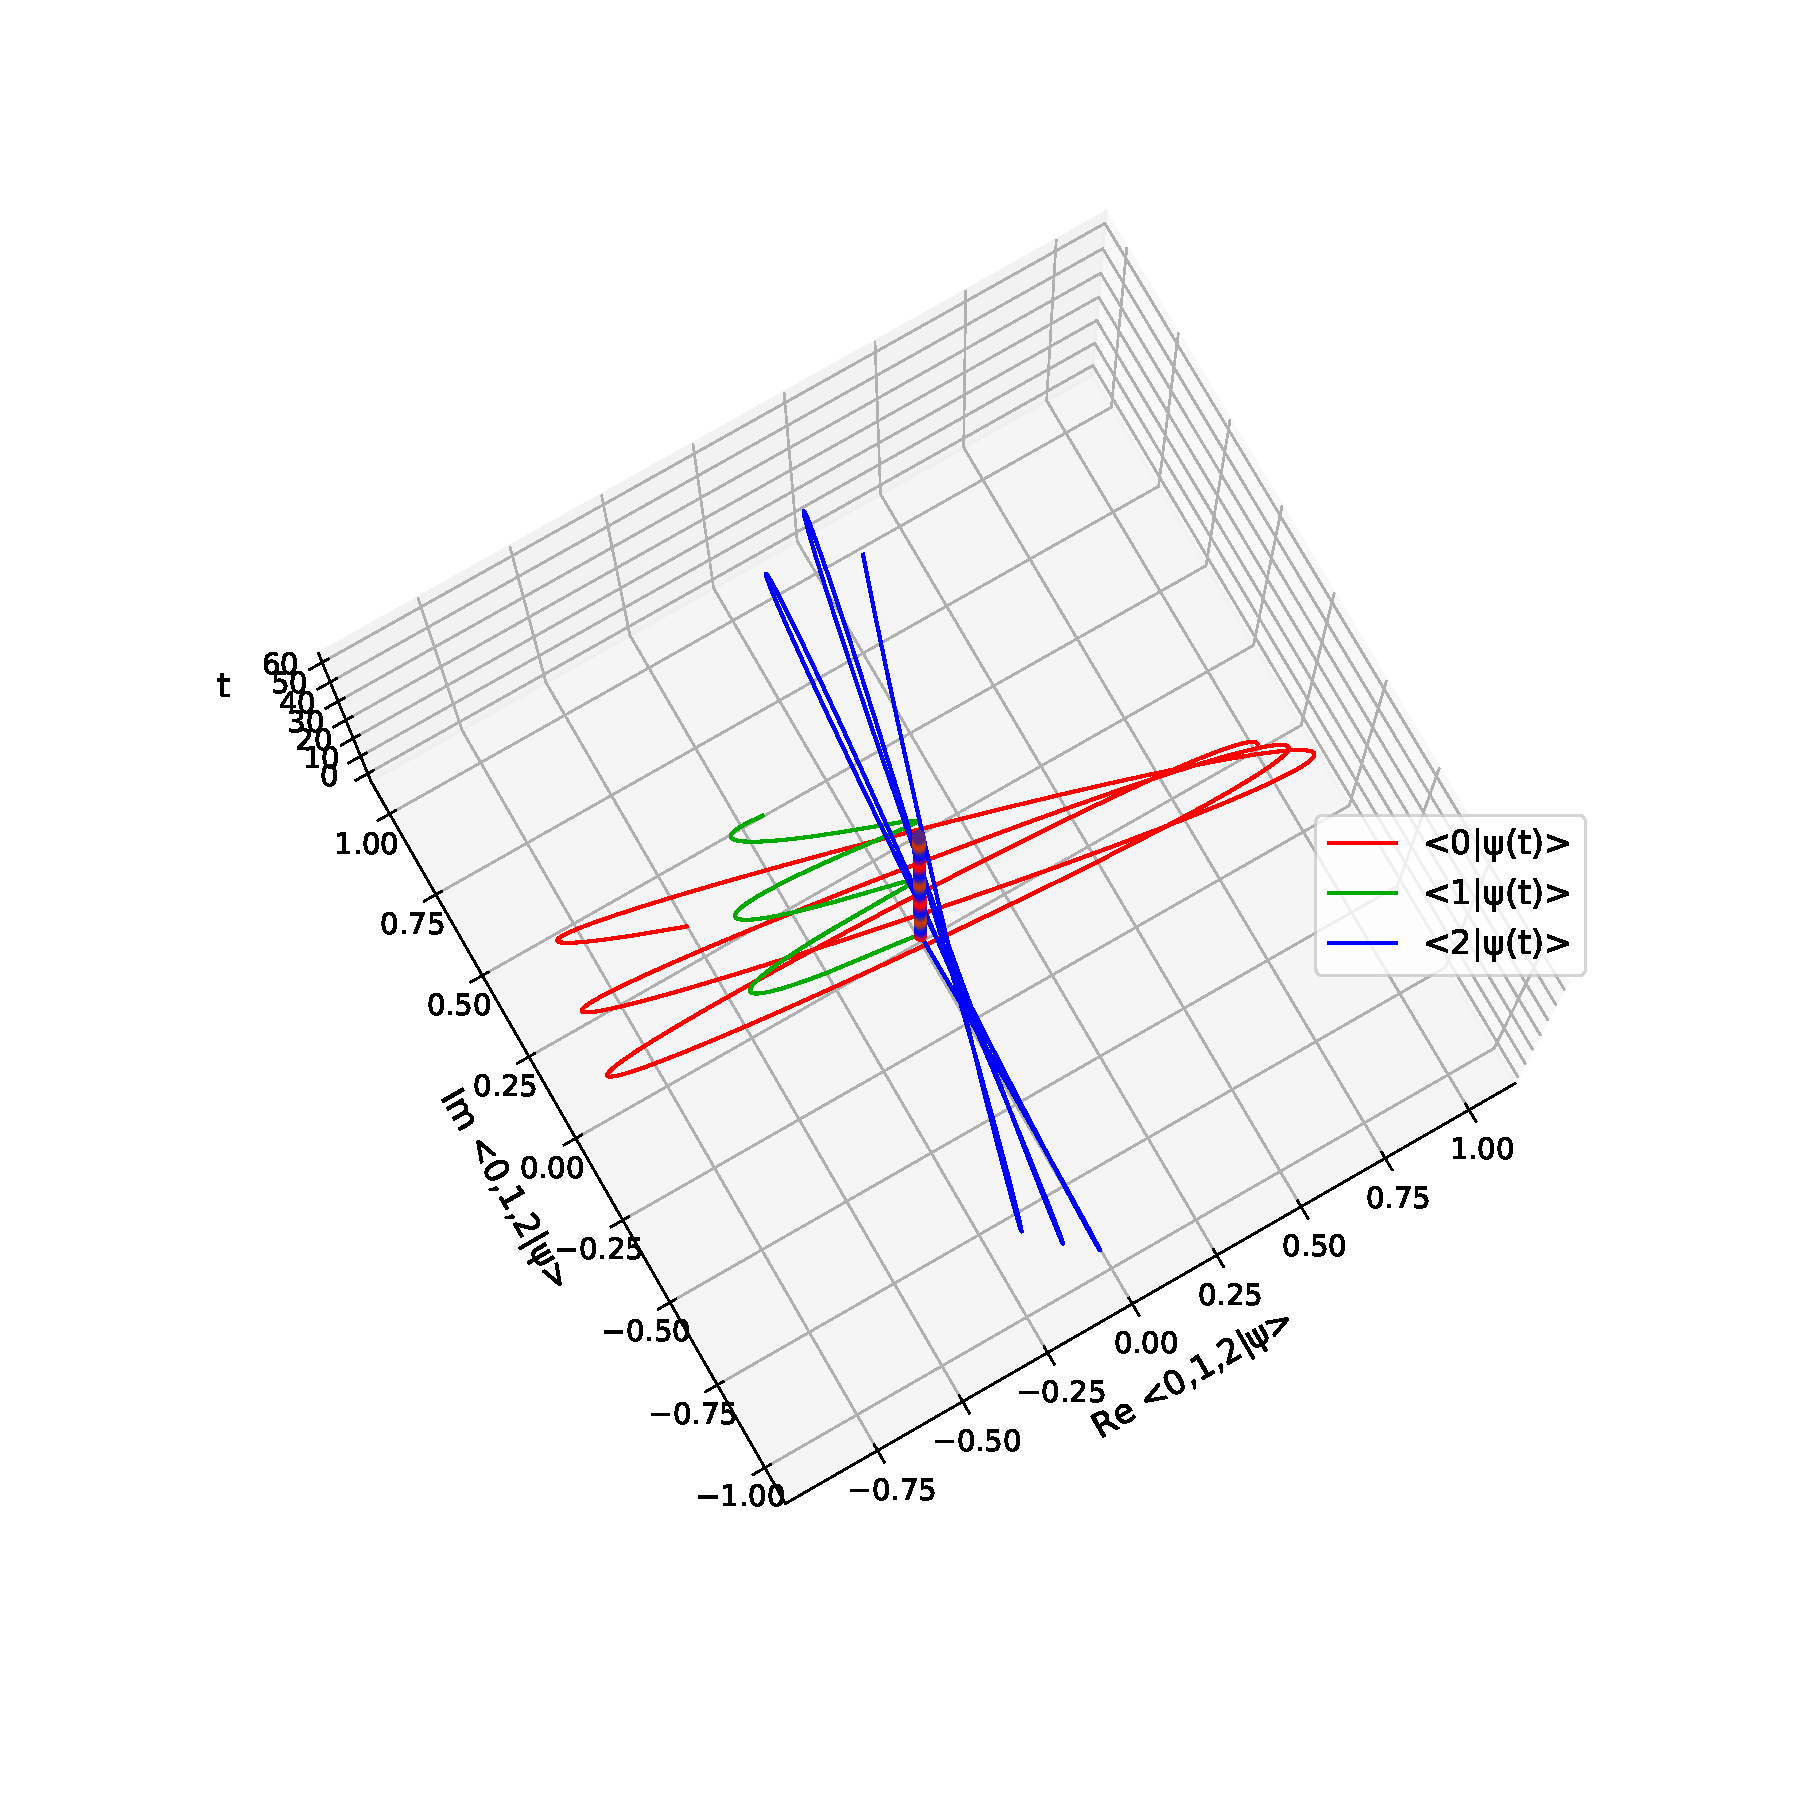
\includegraphics[height=0.41\textheight,clip,trim= 20 120 20 220]{img/3ldetect/hermitianSpaceTime_top.pdf}
    \caption{Bar.}
  \end{subfigure}
  \caption{FooBar.}
  %\label{fig:psi_V}
\end{figure}

% Pobabilities (non-Hermitian) and loss of normalization

\begin{figure}[h]
  \begin{subfigure}[b]{\textwidth}
    \centering
    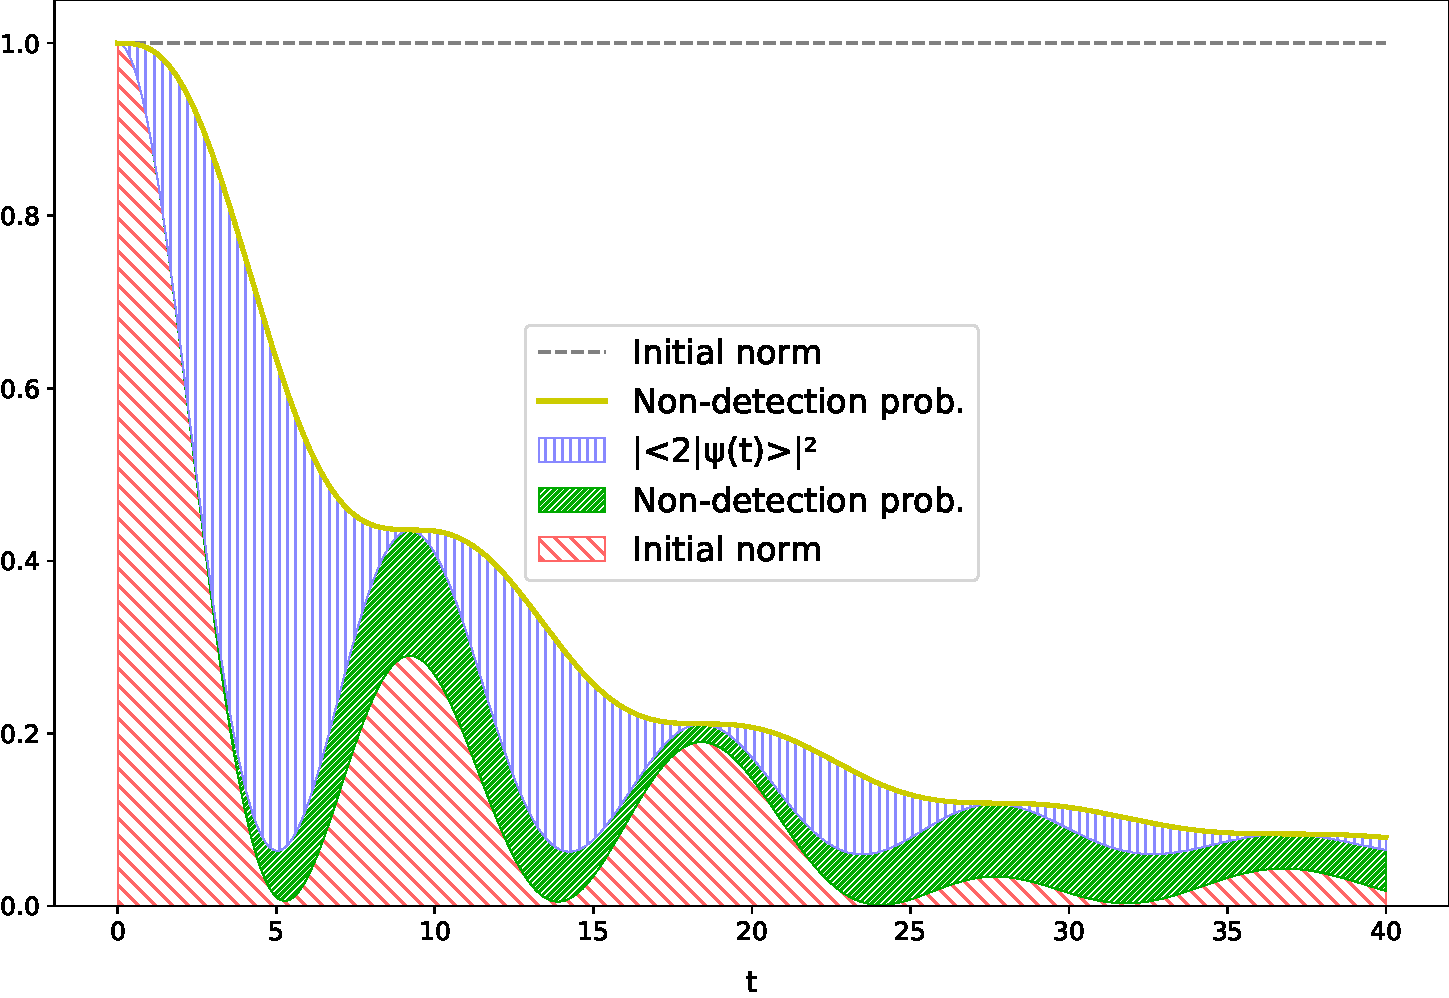
\includegraphics[width=.8\textwidth]{img/3ldetect/loss3color.pdf}
    \subcaption{Foo.}%\label{fig:aabsorbed-qubit-components_pwlattice:re0}
  \end{subfigure}
  \par\bigskip
  \par\bigskip
  \begin{subfigure}[b]{\textwidth}
    \centering
    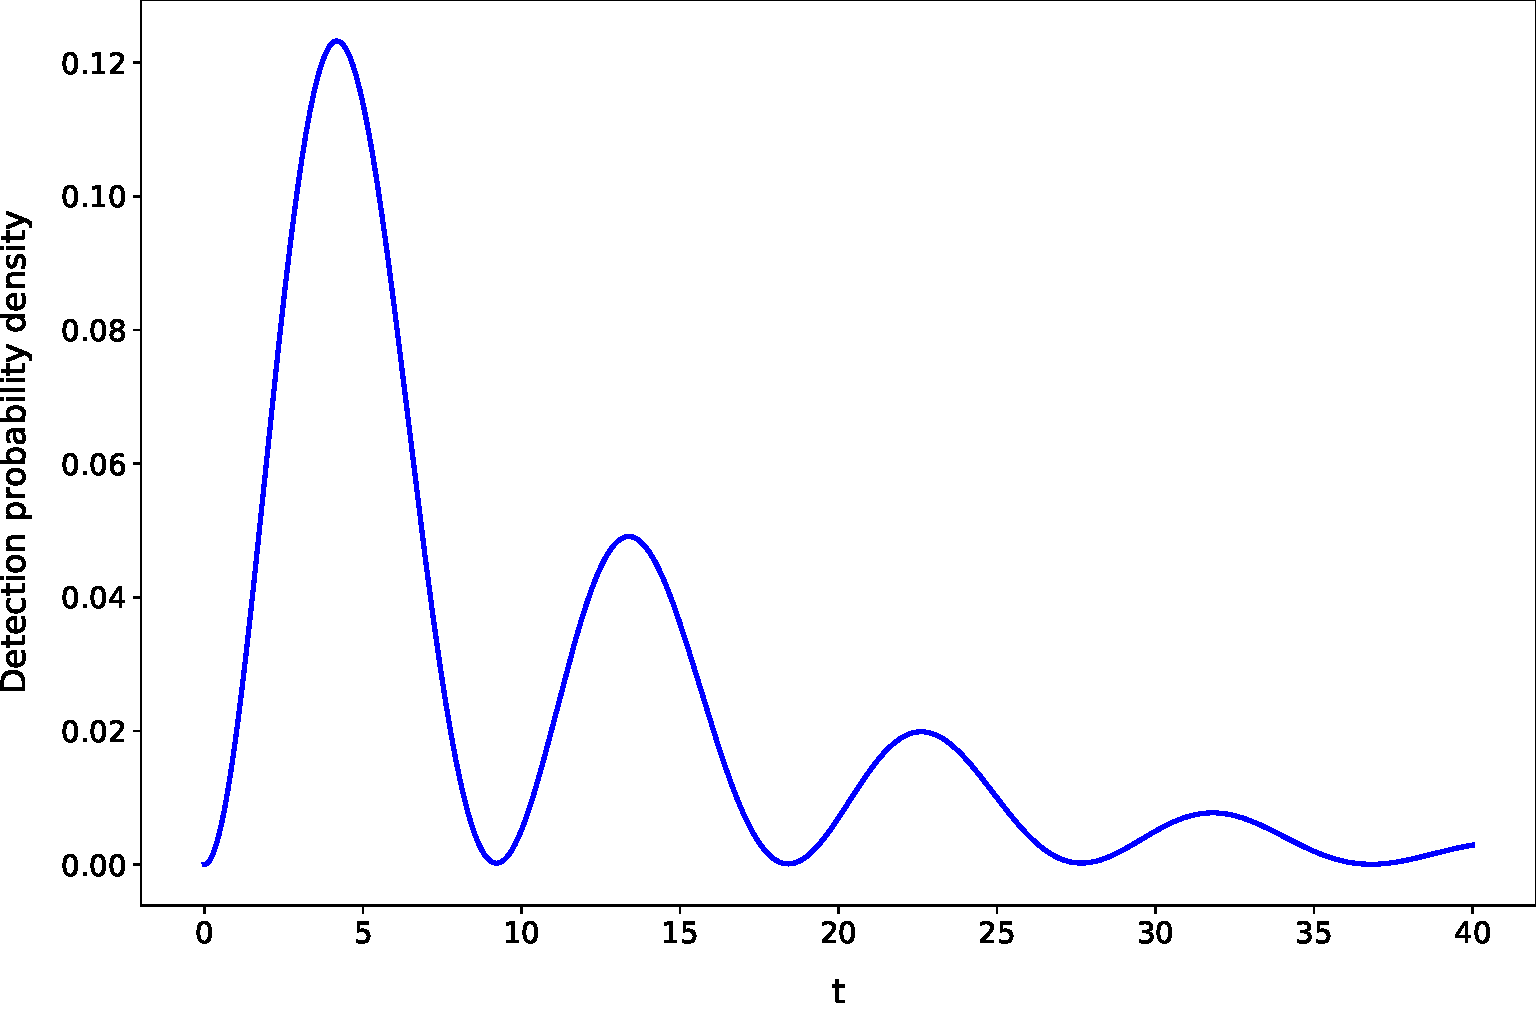
\includegraphics[width=.8\textwidth]{img/3ldetect/loss.pdf}
    \subcaption{Bar.}%\label{fig:aabsorbed-qubit-components_pwlattice:im1}
  \end{subfigure}
  \par\bigskip
  \par\bigskip
  \caption{
    Blah blah blah.
  }
  %\label{fig:aabsorbed-qubit-components_pwlattice}
\end{figure}

% extended time

\begin{figure}[h]
  \begin{subfigure}[b]{\textwidth}
    \centering
    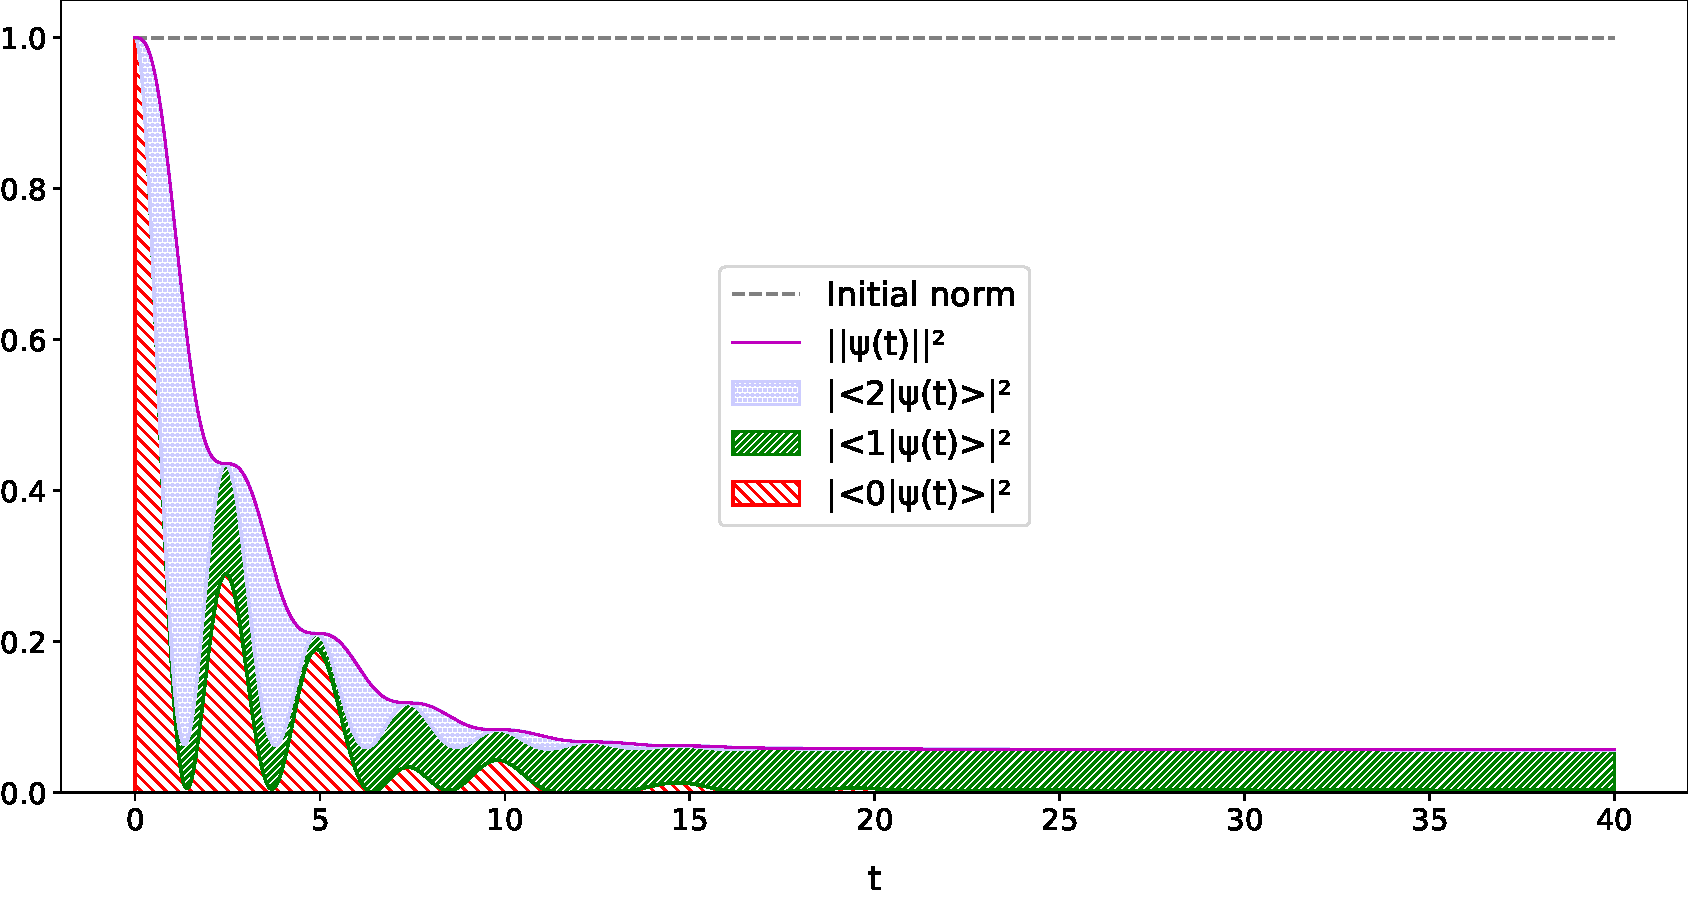
\includegraphics[width=\textwidth]{img/3ldetect/loss3color_ext.pdf}
    \subcaption{Foo.}%\label{fig:aabsorbed-qubit-components_pwlattice:re0}
  \end{subfigure}
  \par\bigskip
  \par\bigskip
  \begin{subfigure}[b]{\textwidth}
    \centering
    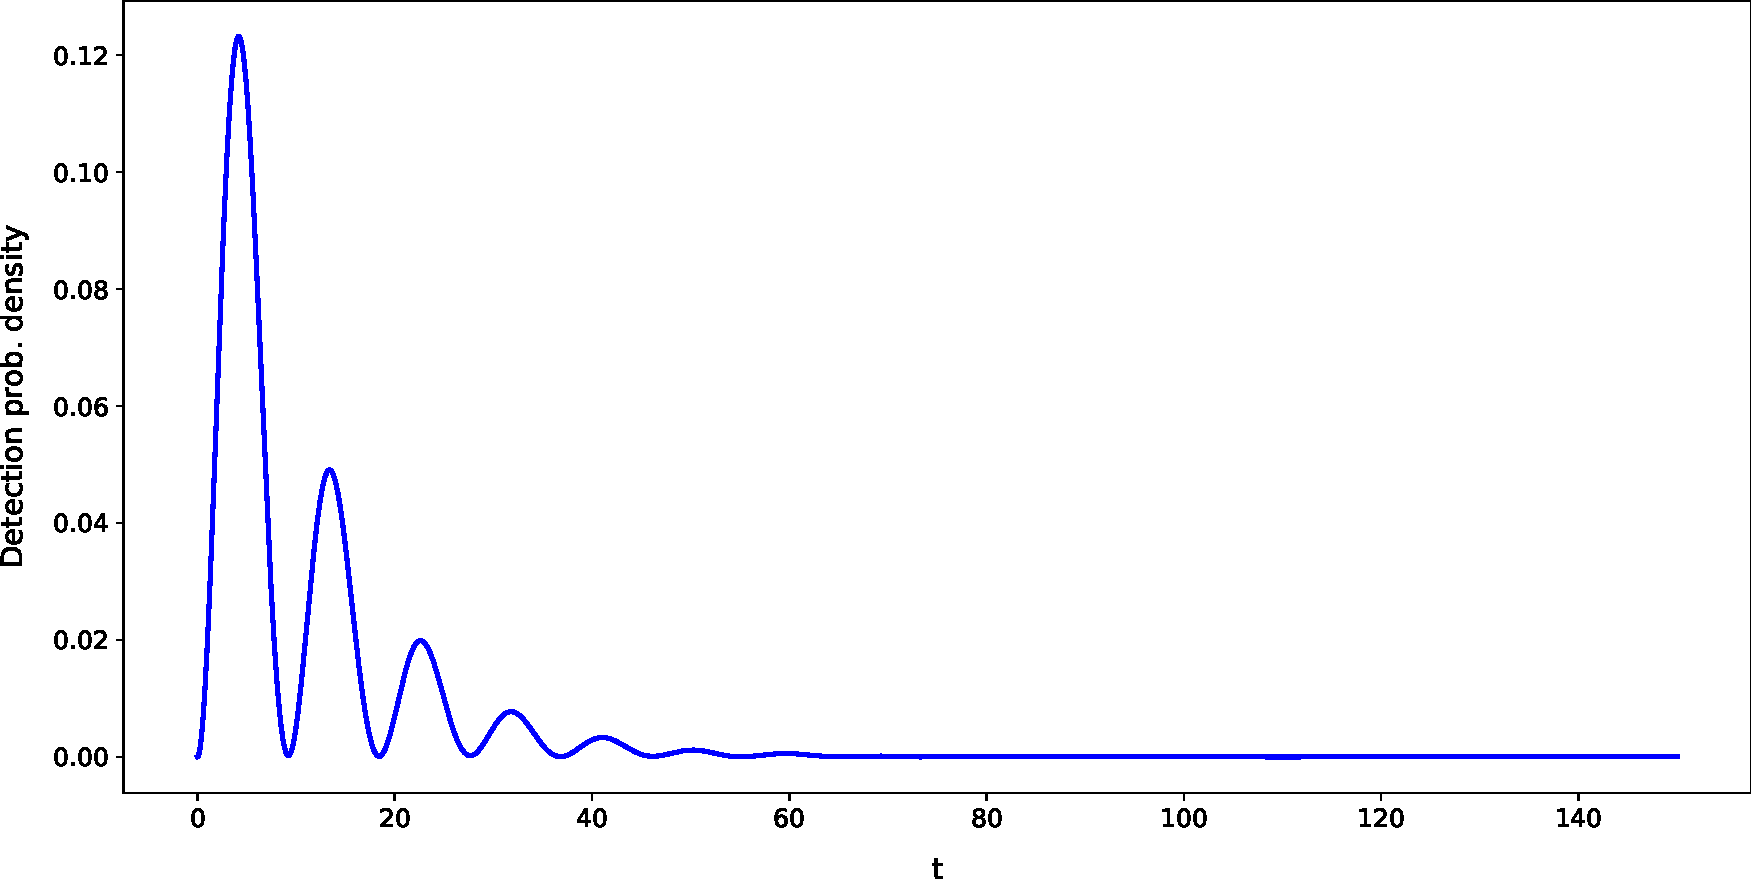
\includegraphics[width=\textwidth]{img/3ldetect/loss_ext.pdf}
    \subcaption{Bar.}%\label{fig:aabsorbed-qubit-components_pwlattice:im1}
  \end{subfigure}
  \par\bigskip
  \par\bigskip
  \caption{
    Blah blah blah.
  }
  %\label{fig:aabsorbed-qubit-components_pwlattice}
\end{figure}

% "3D"

\begin{figure}[h]
  \begin{subfigure}[b]{\textwidth}
    \centering
    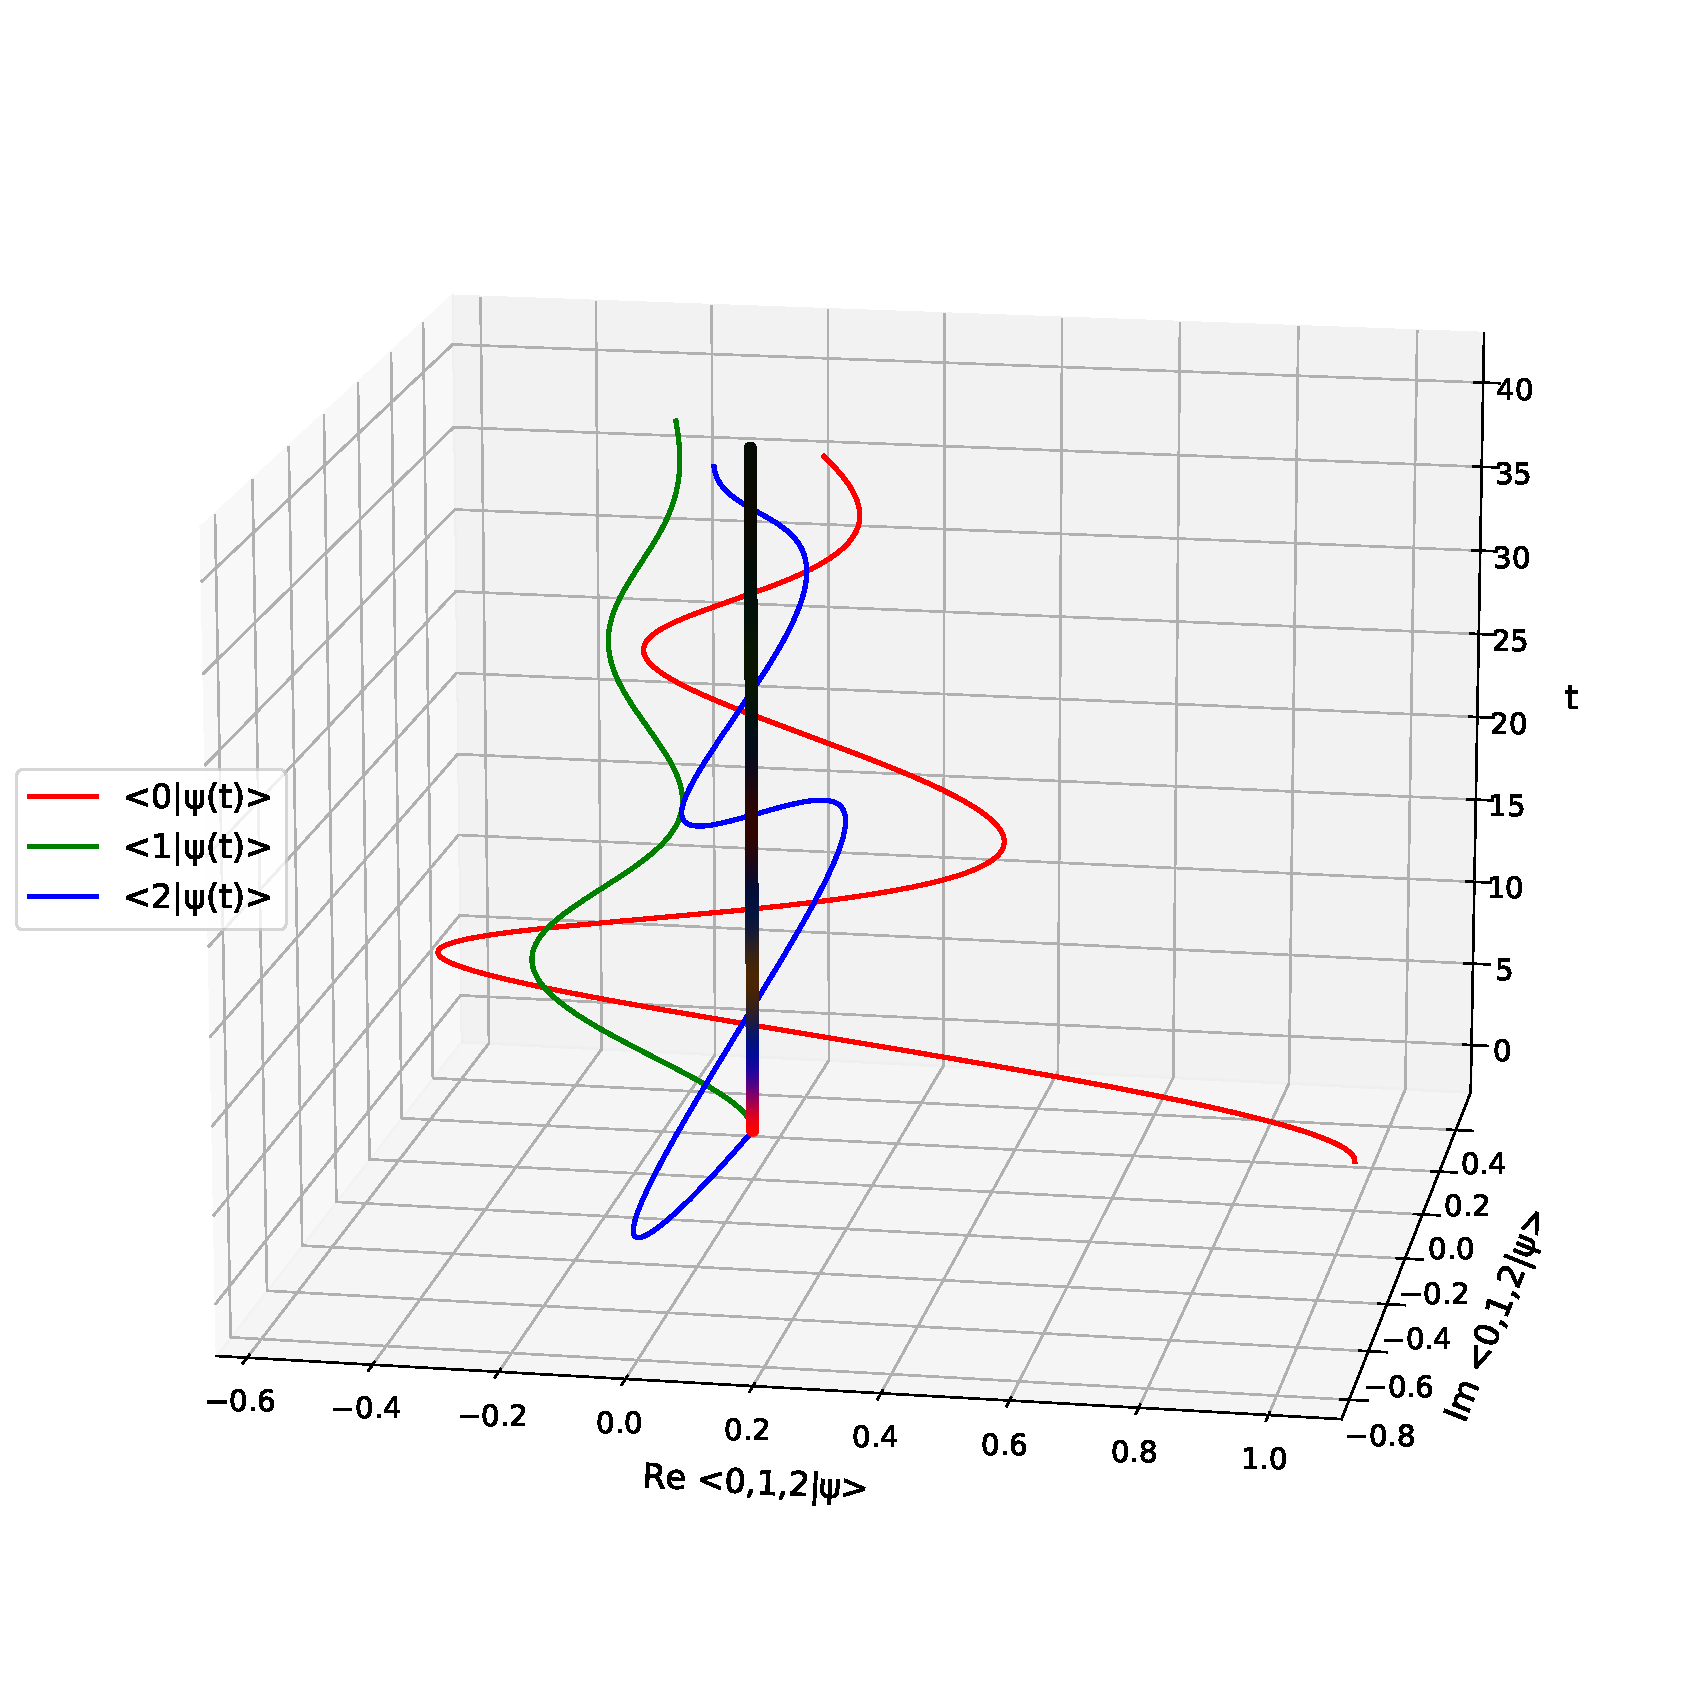
\includegraphics[height=0.41\textheight,clip,trim=0 90 40 140]{img/3ldetect/NonHermitianSpaceTime_side.pdf}
    \caption{Foo.}
  \end{subfigure}
  \par\bigskip
  \begin{subfigure}[b]{\textwidth}
    \centering
    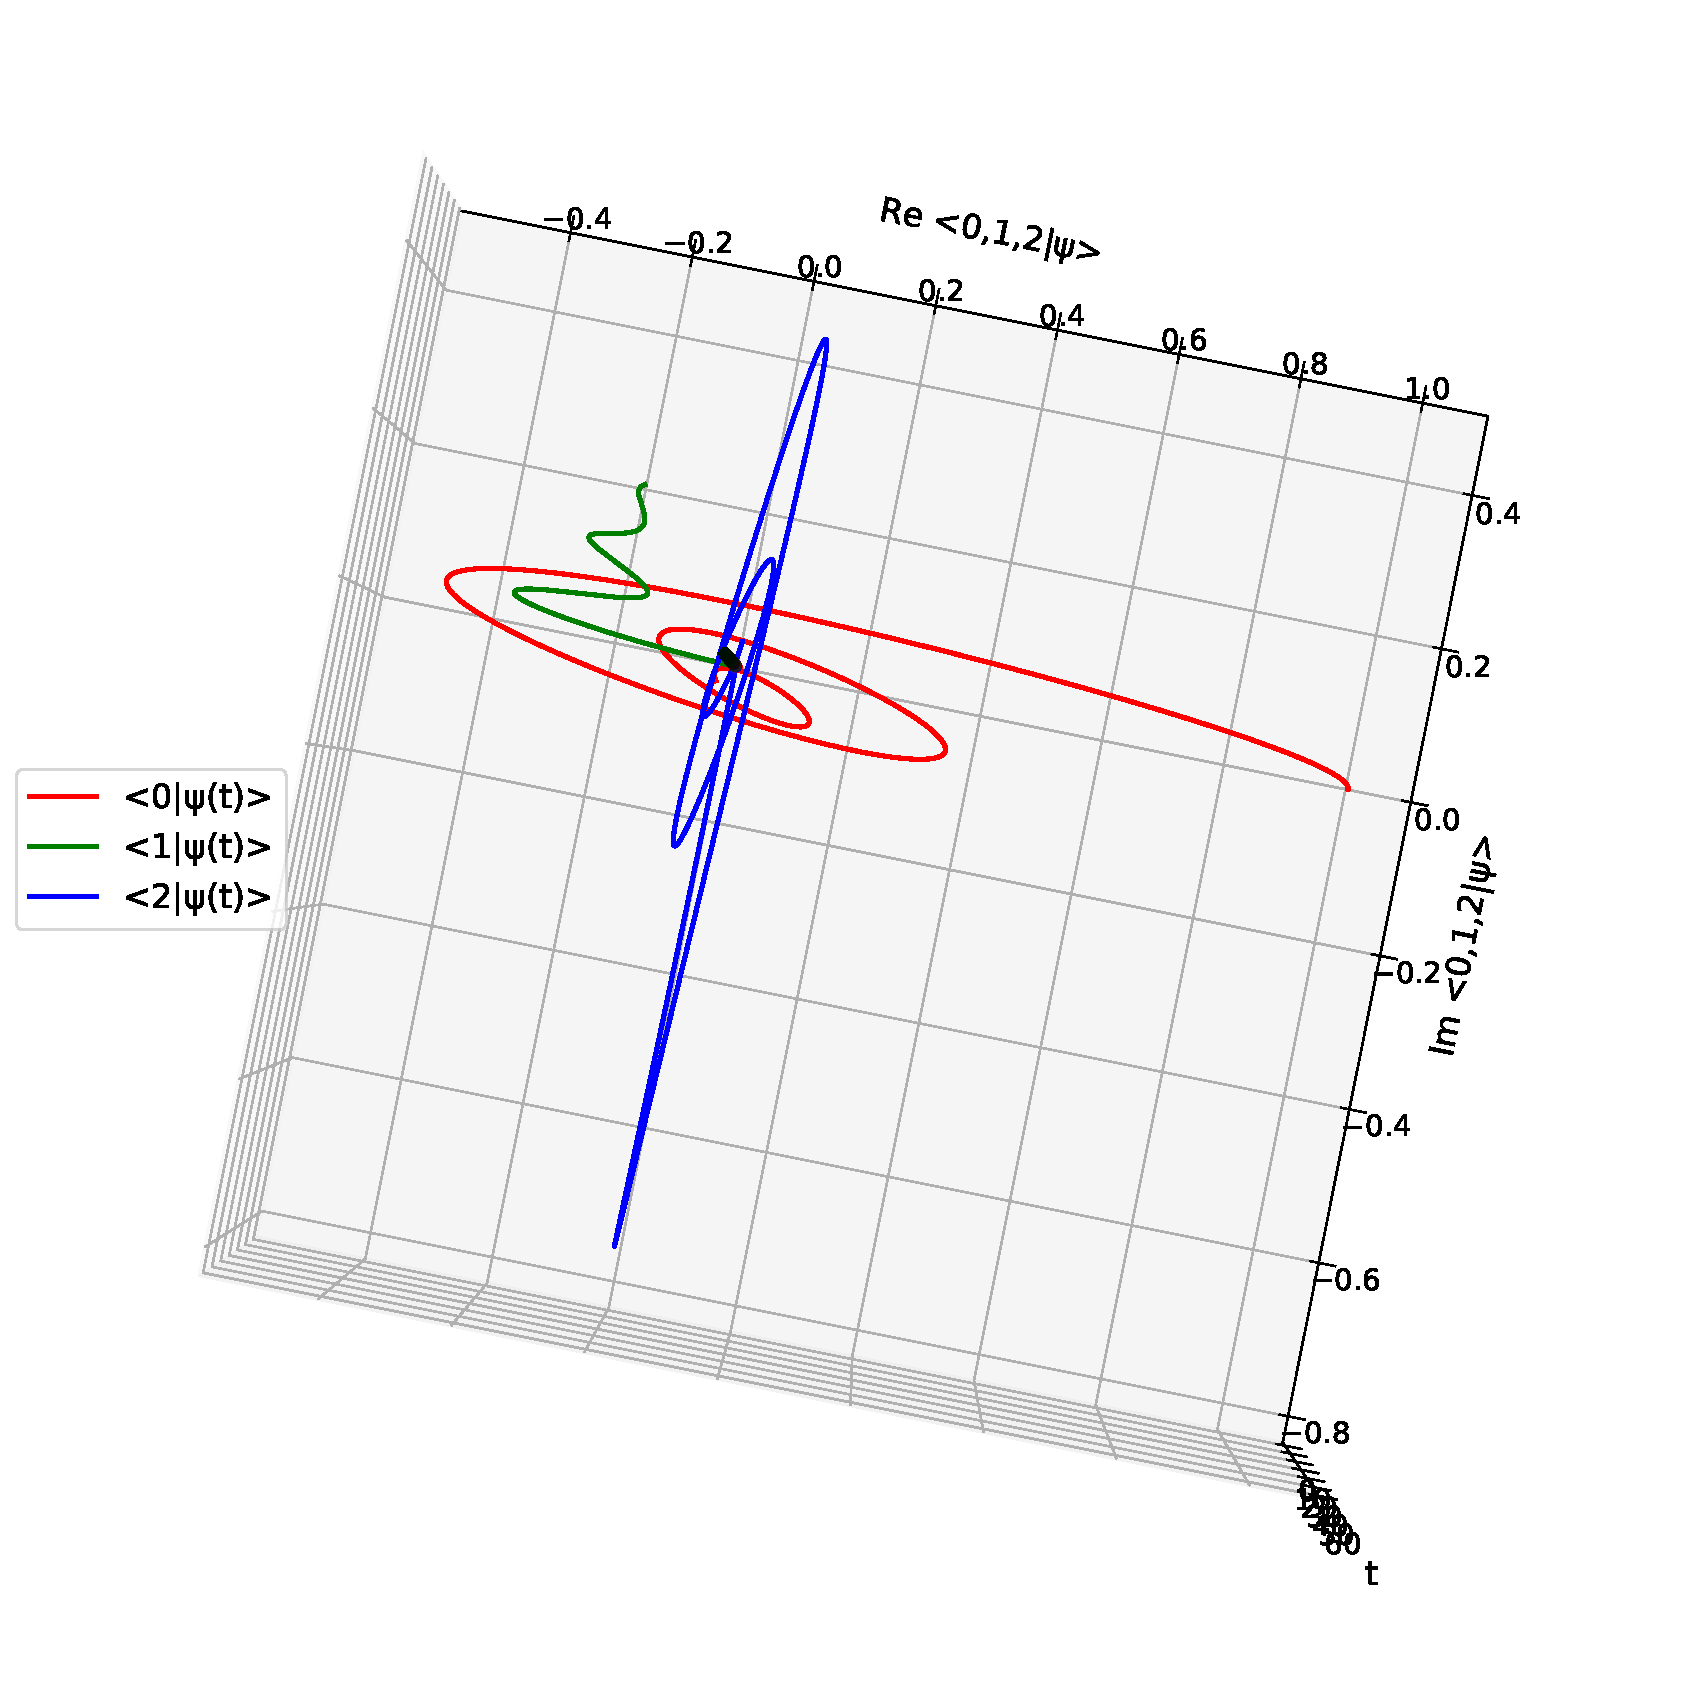
\includegraphics[height=0.44\textheight,clip,trim= 0 90 20 75]{img/3ldetect/NonHermitianSpaceTime_top.pdf}
    \caption{Bar.}
  \end{subfigure}
  \caption{FooBar.}
  %\label{fig:psi_V}
\end{figure}

% P-W

\begin{figure}[h]
  \begin{subfigure}[b]{\textwidth}
    \centering
    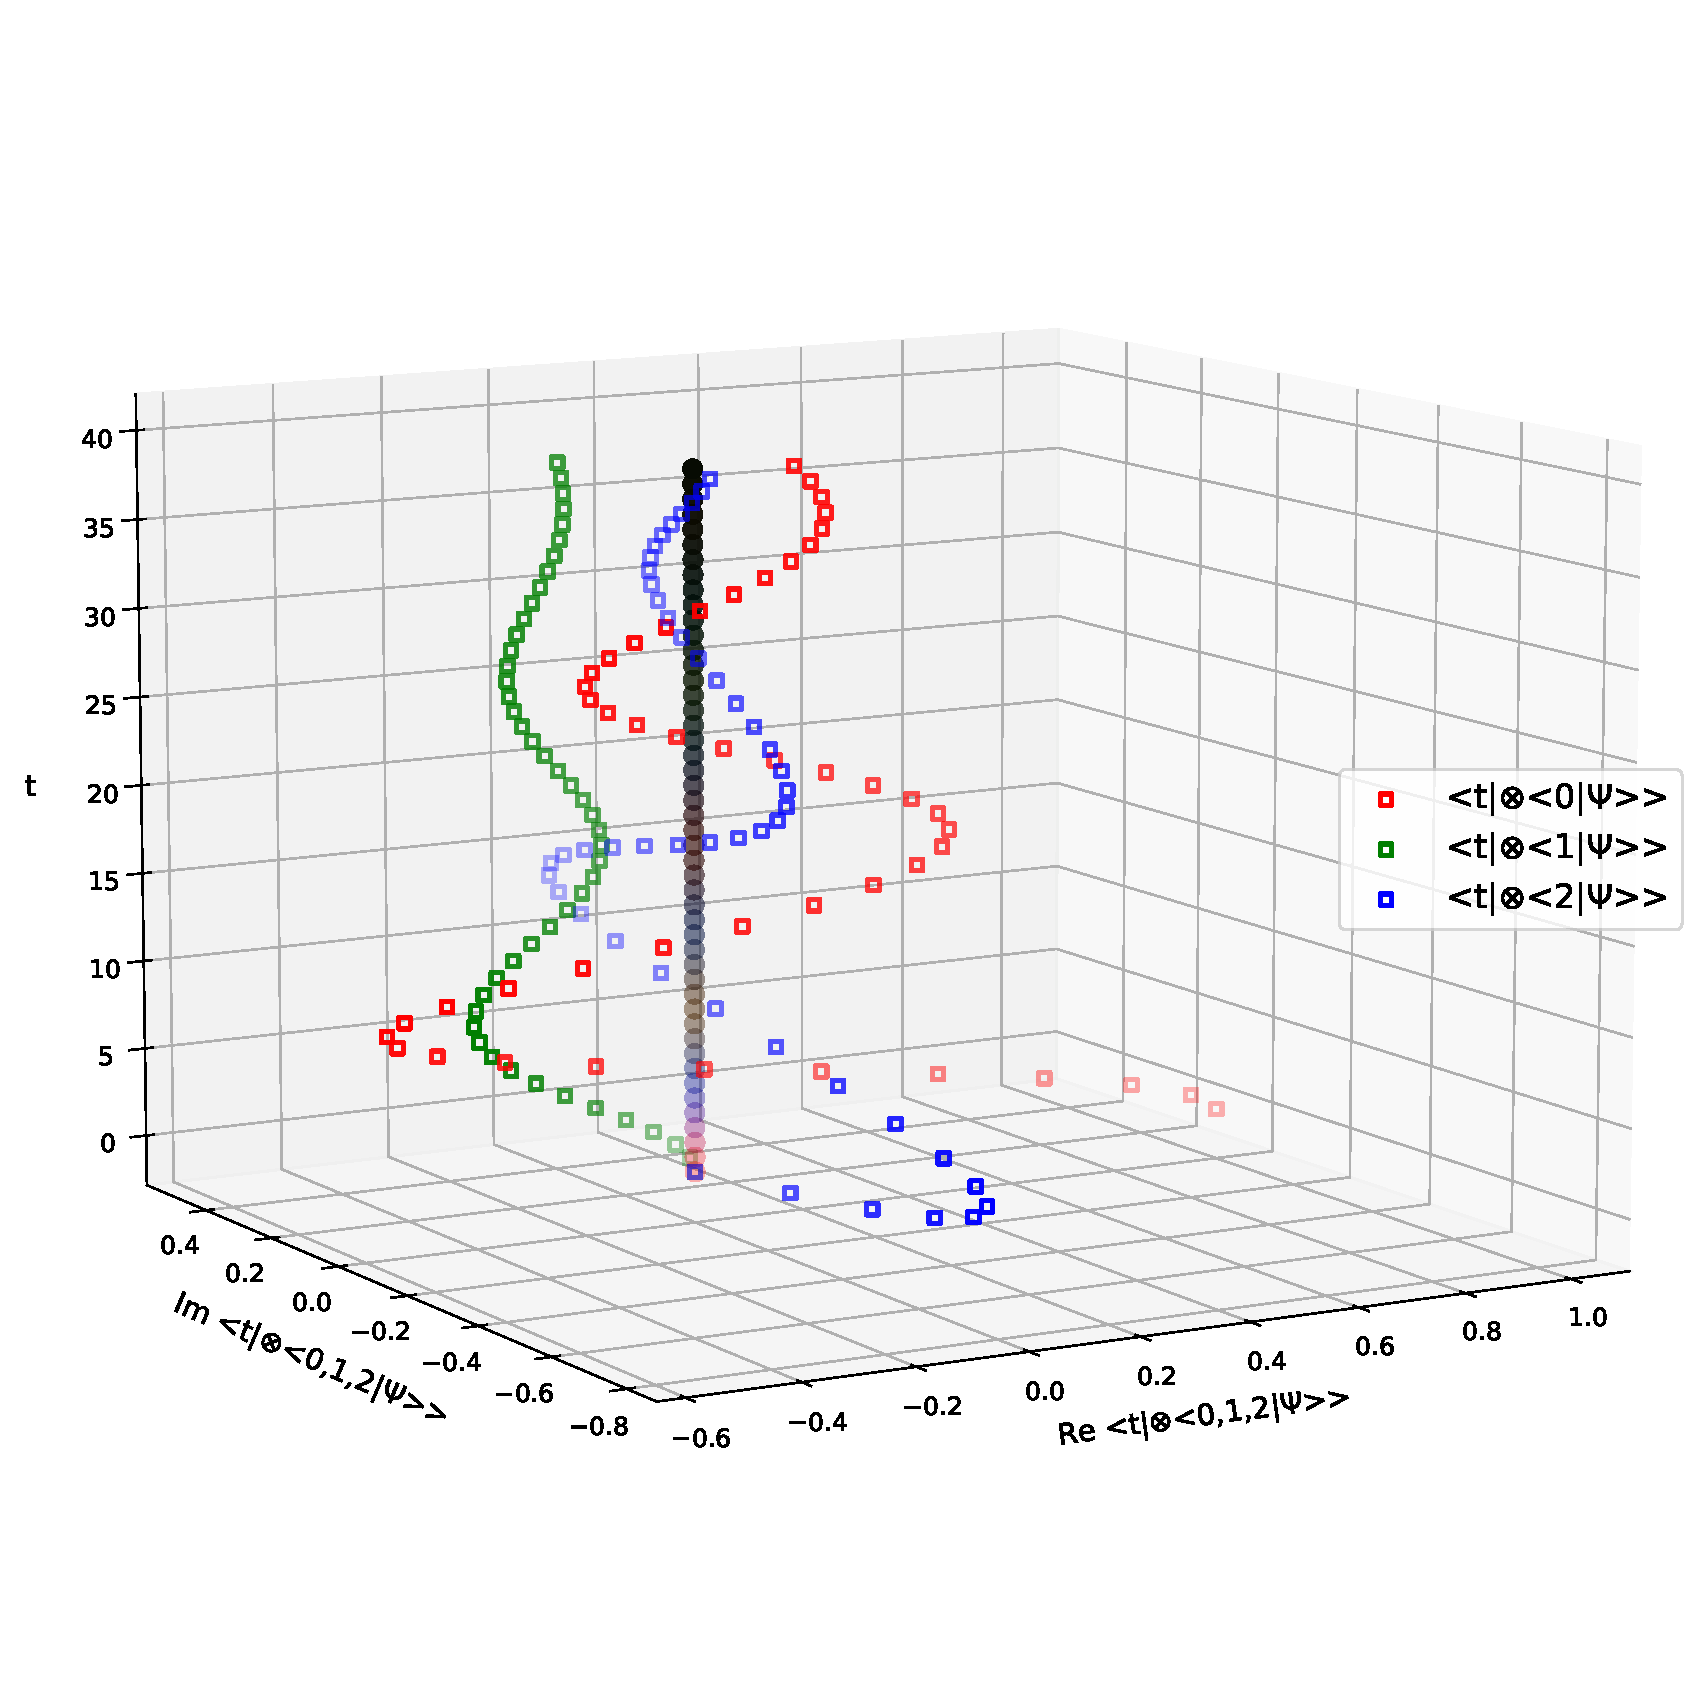
\includegraphics[height=0.41\textheight,clip,trim=0 90 0 140]{img/3ldetect/PWSpaceTime_side.pdf}
    \caption{Foo.}
  \end{subfigure}
  \par\bigskip
  \begin{subfigure}[b]{\textwidth}
    \centering
    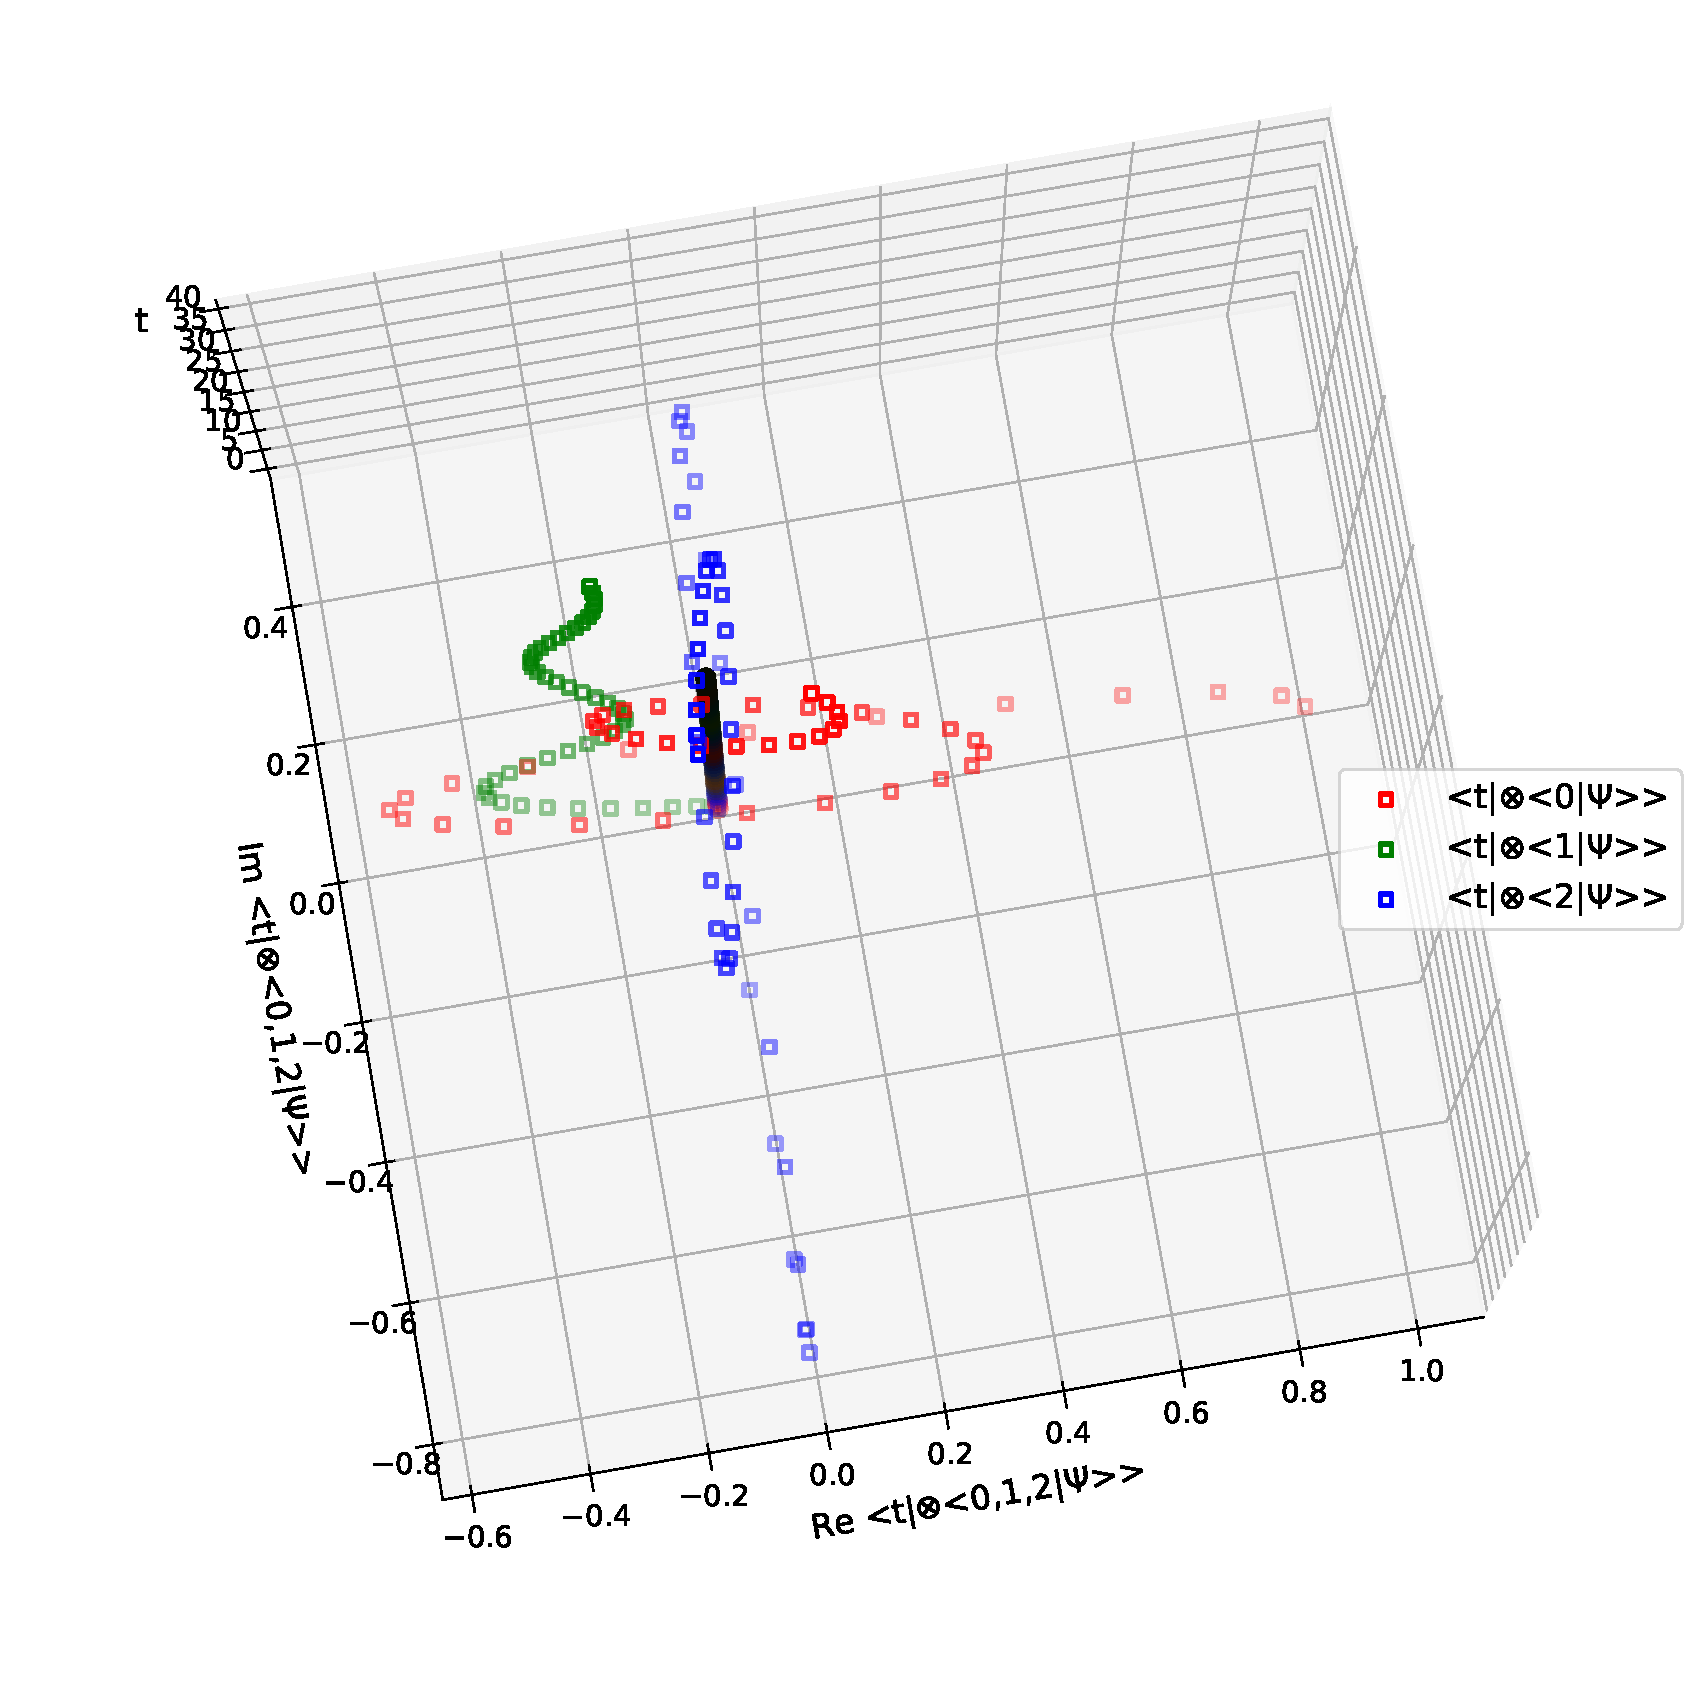
\includegraphics[height=0.48\textheight,clip,trim= 0 60 0 100]{img/3ldetect/PWSpaceTime_top.pdf}
    \caption{Bar.}
  \end{subfigure}
  \caption{FooBar.}
  %\label{fig:psi_V}
\end{figure}

% P-W vs QM

% \begin{figure}[h]
%   \begin{subfigure}[b]{\textwidth}
%     \centering
%     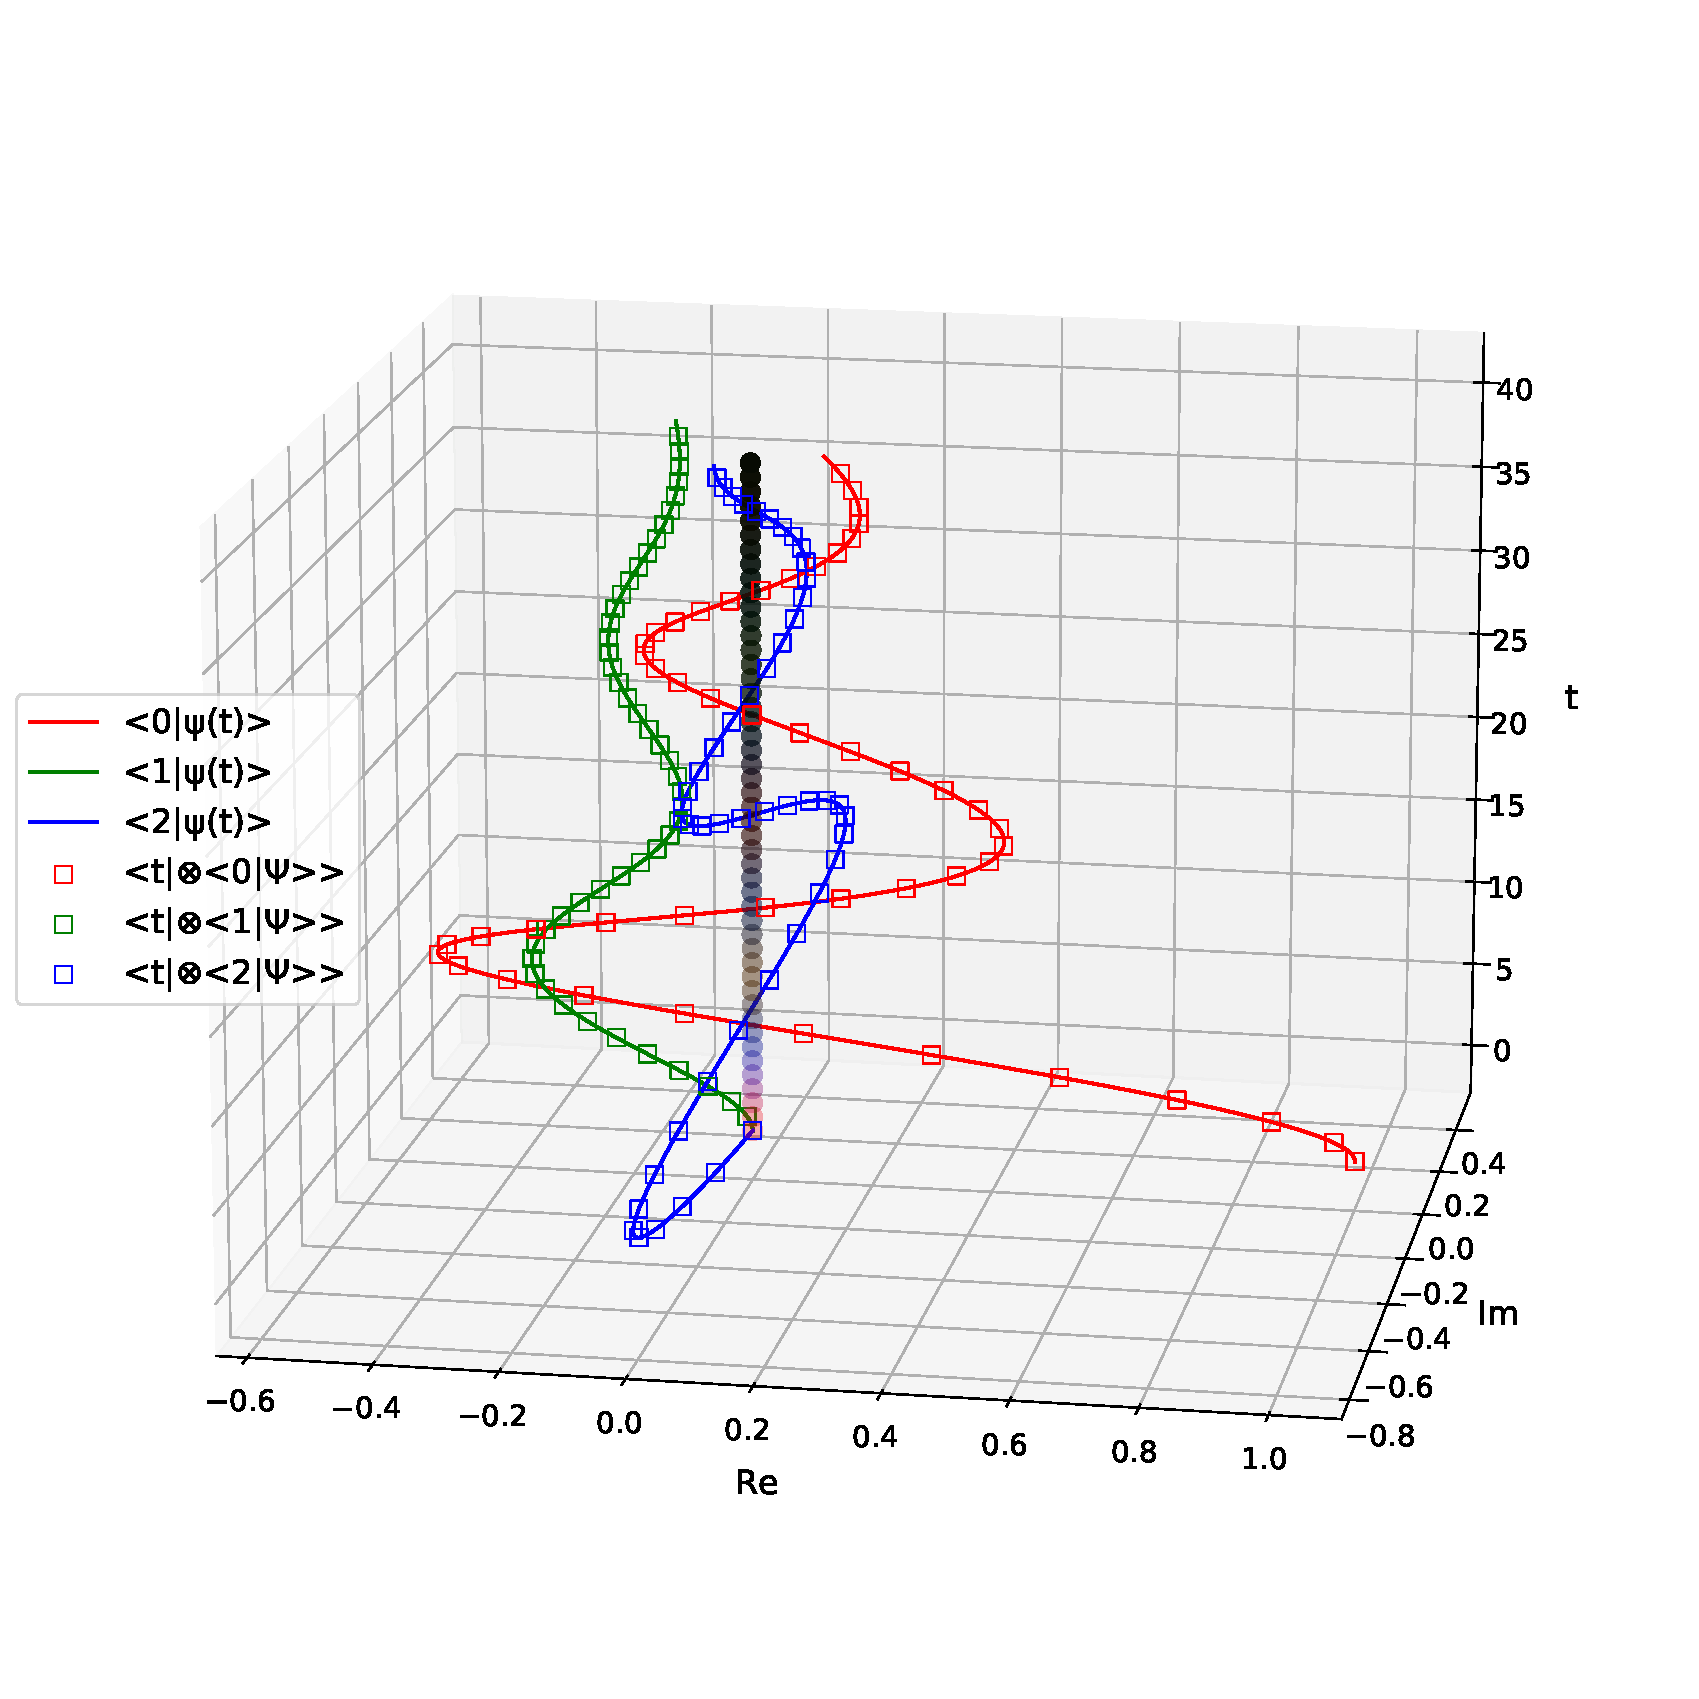
\includegraphics[height=0.41\textheight,clip,trim=0 90 0 140]{img/3ldetect/PWSpaceTimeFit_side.pdf}
%     \caption{Foo.}
%   \end{subfigure}
%   \par\bigskip
%   \begin{subfigure}[b]{\textwidth}
%     \centering
%     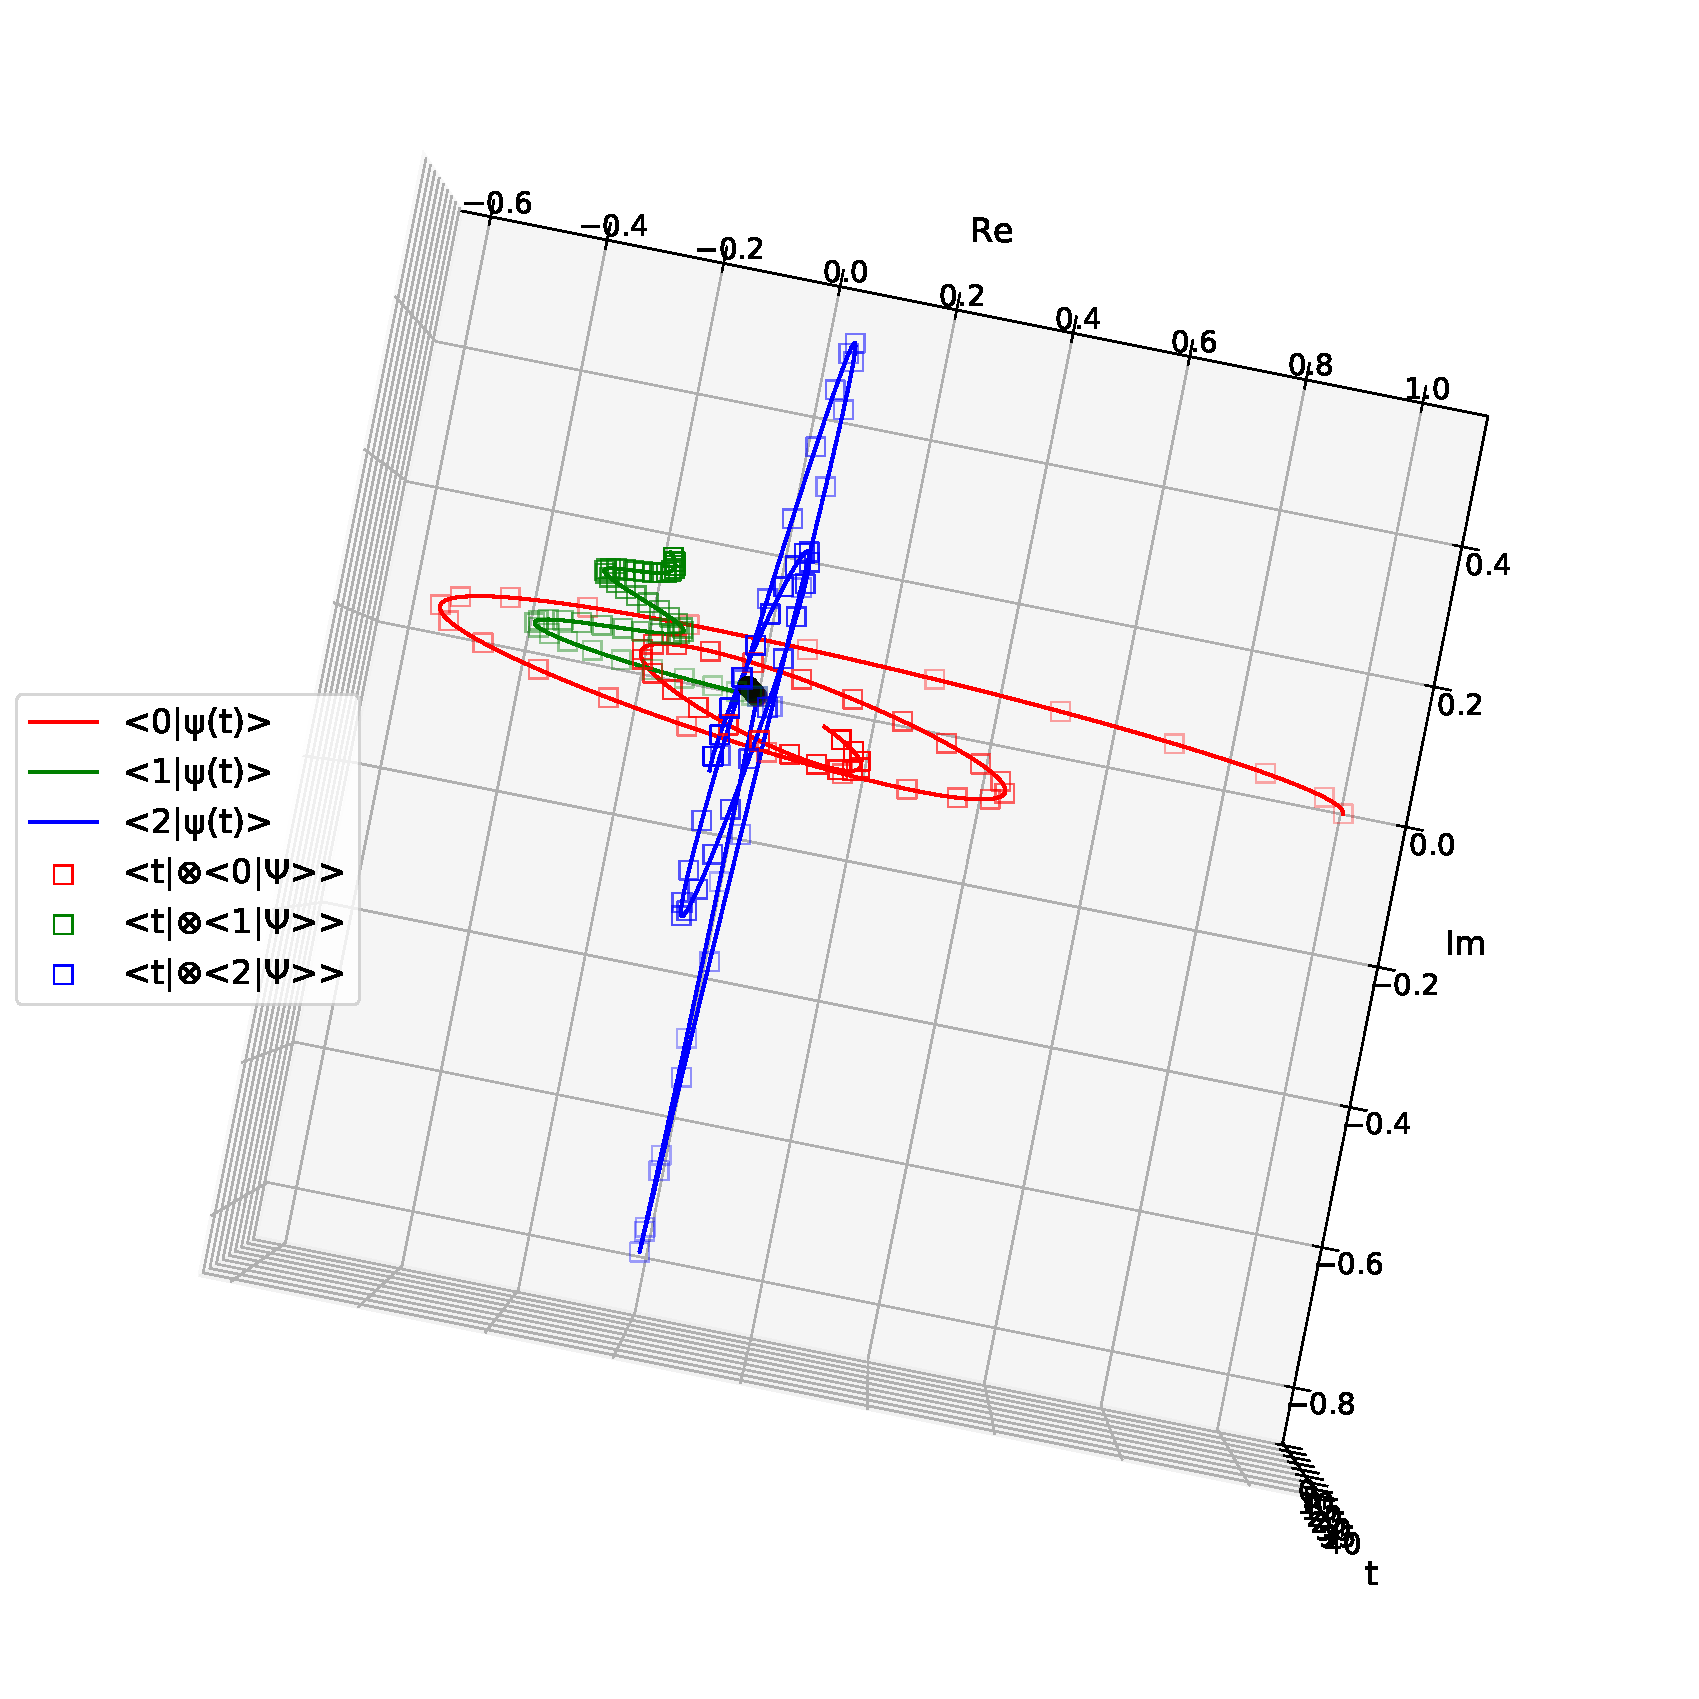
\includegraphics[height=0.48\textheight,clip,trim= 0 60 0 100]{img/3ldetect/PWSpaceTimeFit_top.pdf}
%     \caption{Bar.}
%   \end{subfigure}
%   \caption{FooBar.}
%   %\label{fig:psi_V}
% \end{figure}

\begin{figure}[hb!]
  \centering
  \begin{subfigure}{\textwidth}
      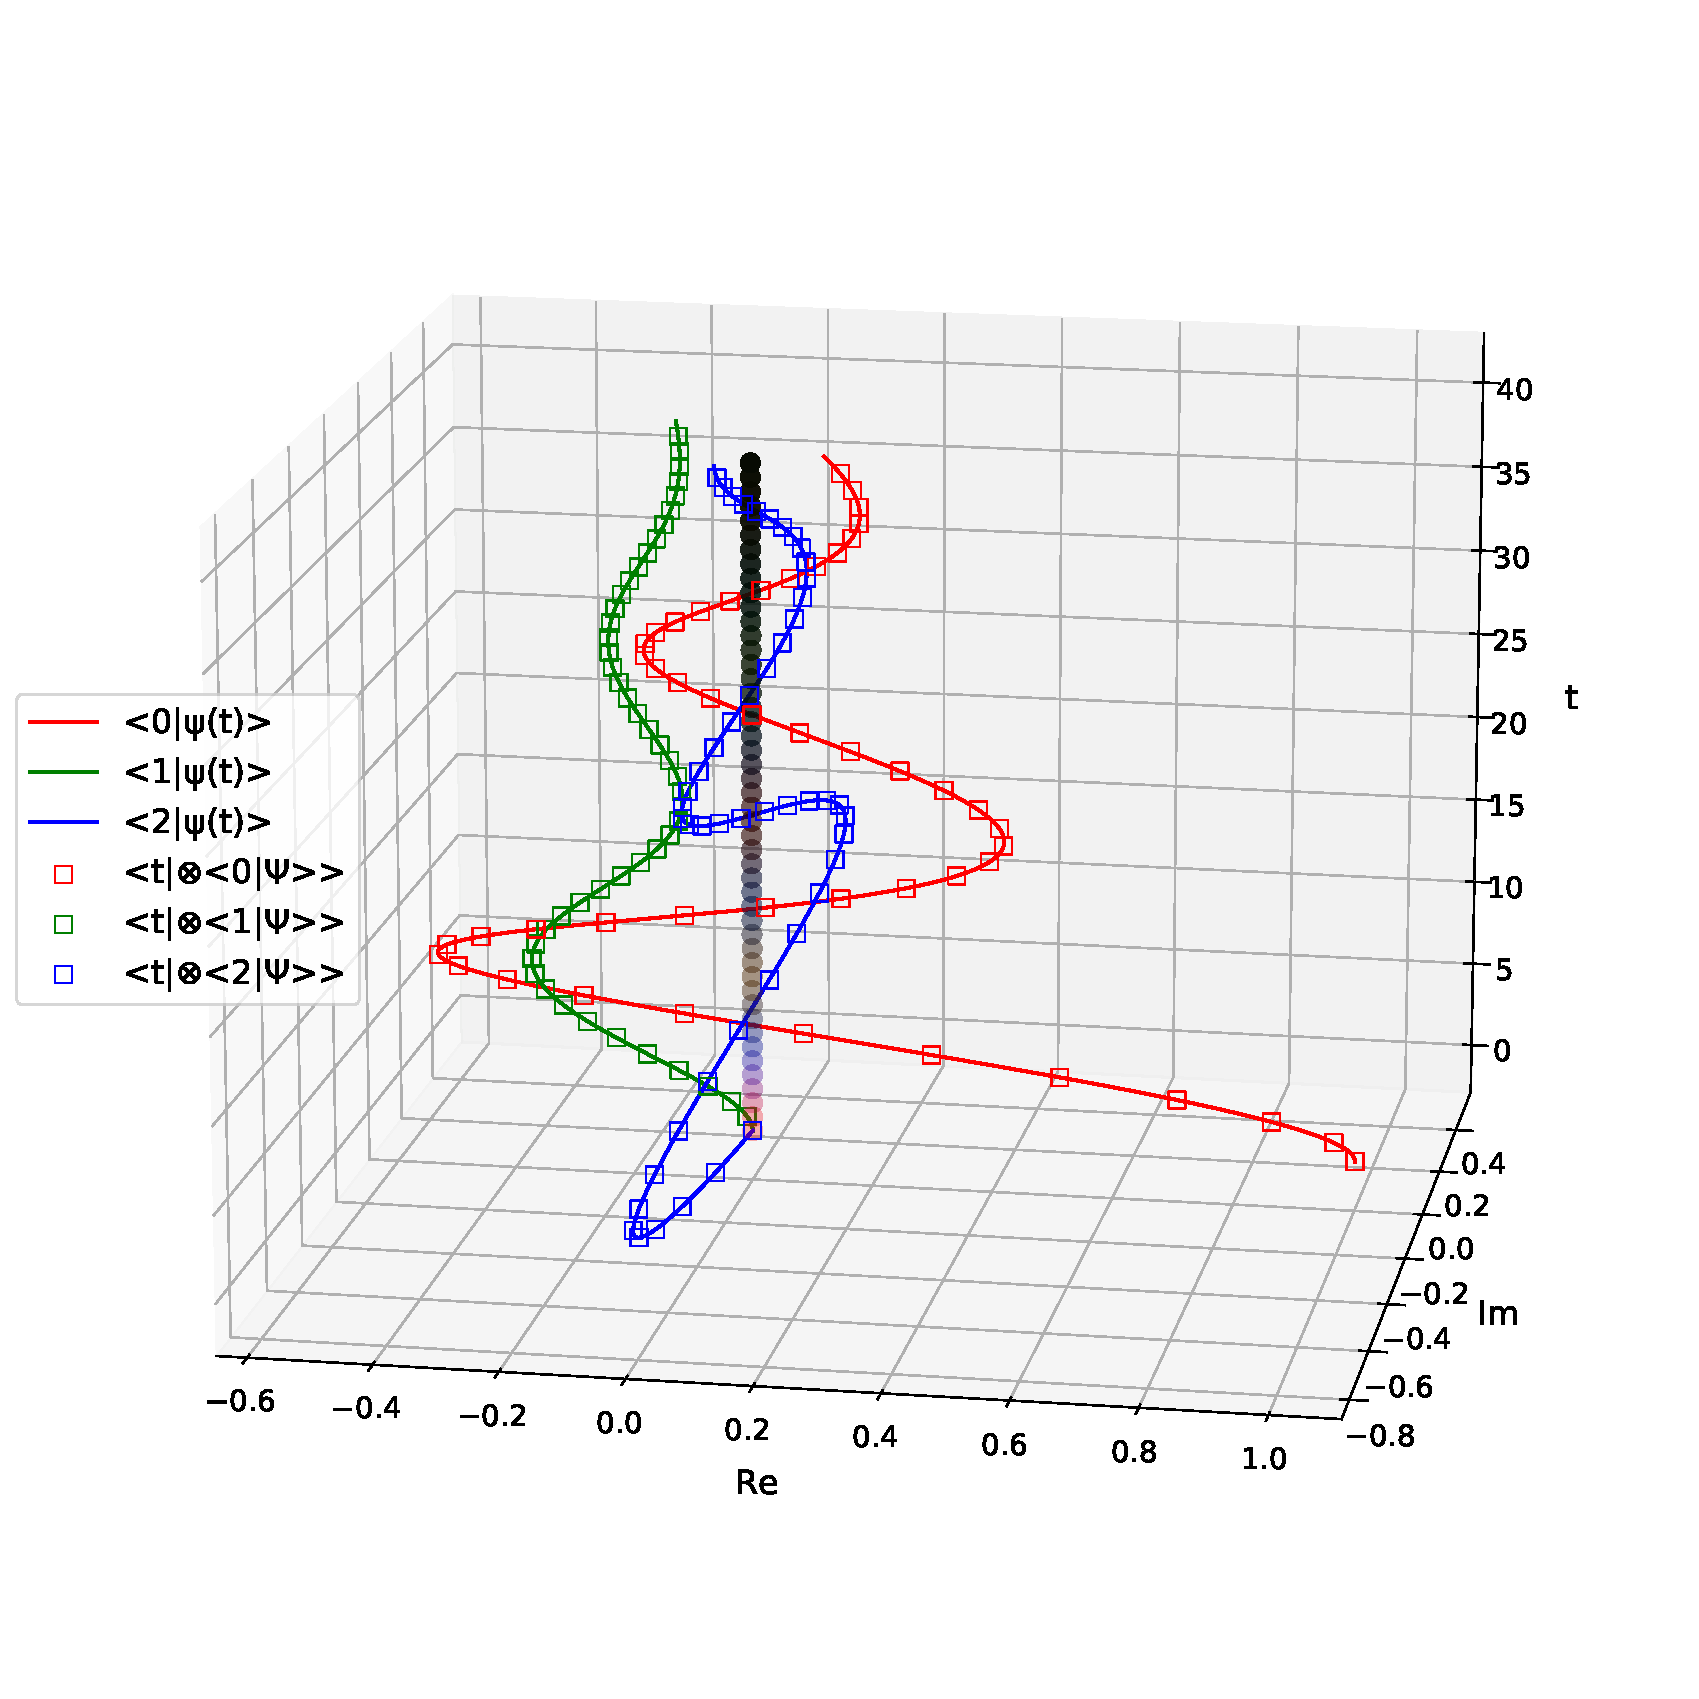
\includegraphics[width=\textwidth]{img/3ldetect/PWSpaceTimeFit_side.pdf}
      \subcaption{Foo.}
      %\label{fig:arm1}
  \end{subfigure}
  \caption{Foobar.}
\end{figure}%
\begin{figure}[ht]\ContinuedFloat
  \centering
  \begin{subfigure}{\textwidth}
      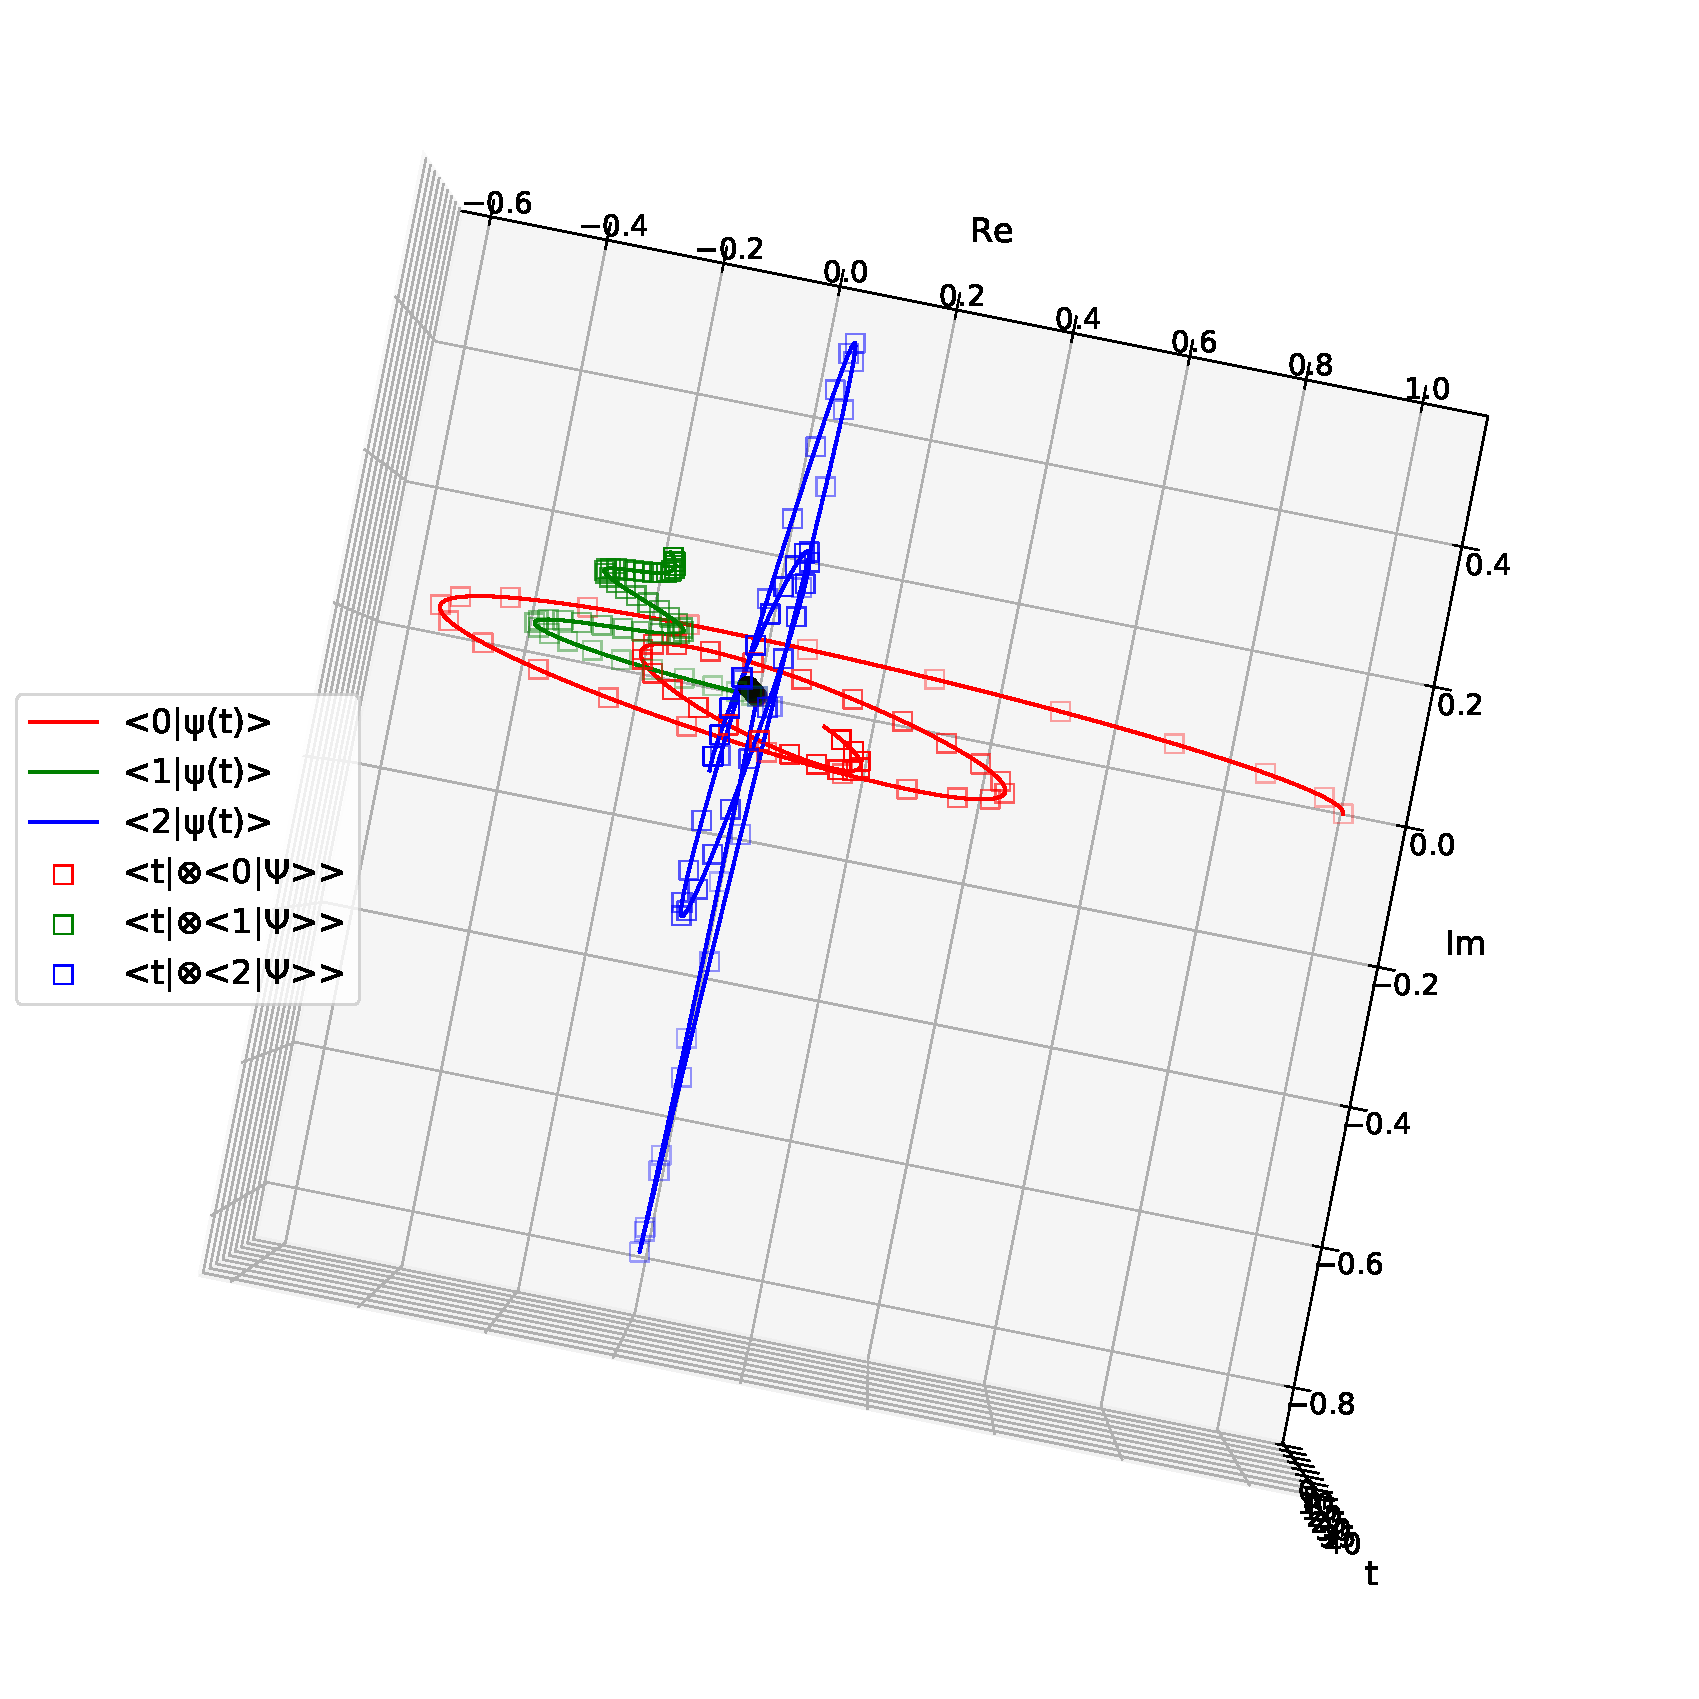
\includegraphics[width=\textwidth]{img/3ldetect/PWSpaceTimeFit_top.pdf}
      \subcaption{Bar.}
      %\label{fig:arm3}
  \end{subfigure}
  \caption{Foobar (cont.)}
\end{figure}

% P-W (bayesian) vs Detector model (norm. loss, Allcock...) detection probability

\begin{figure}[h]
  \centering
  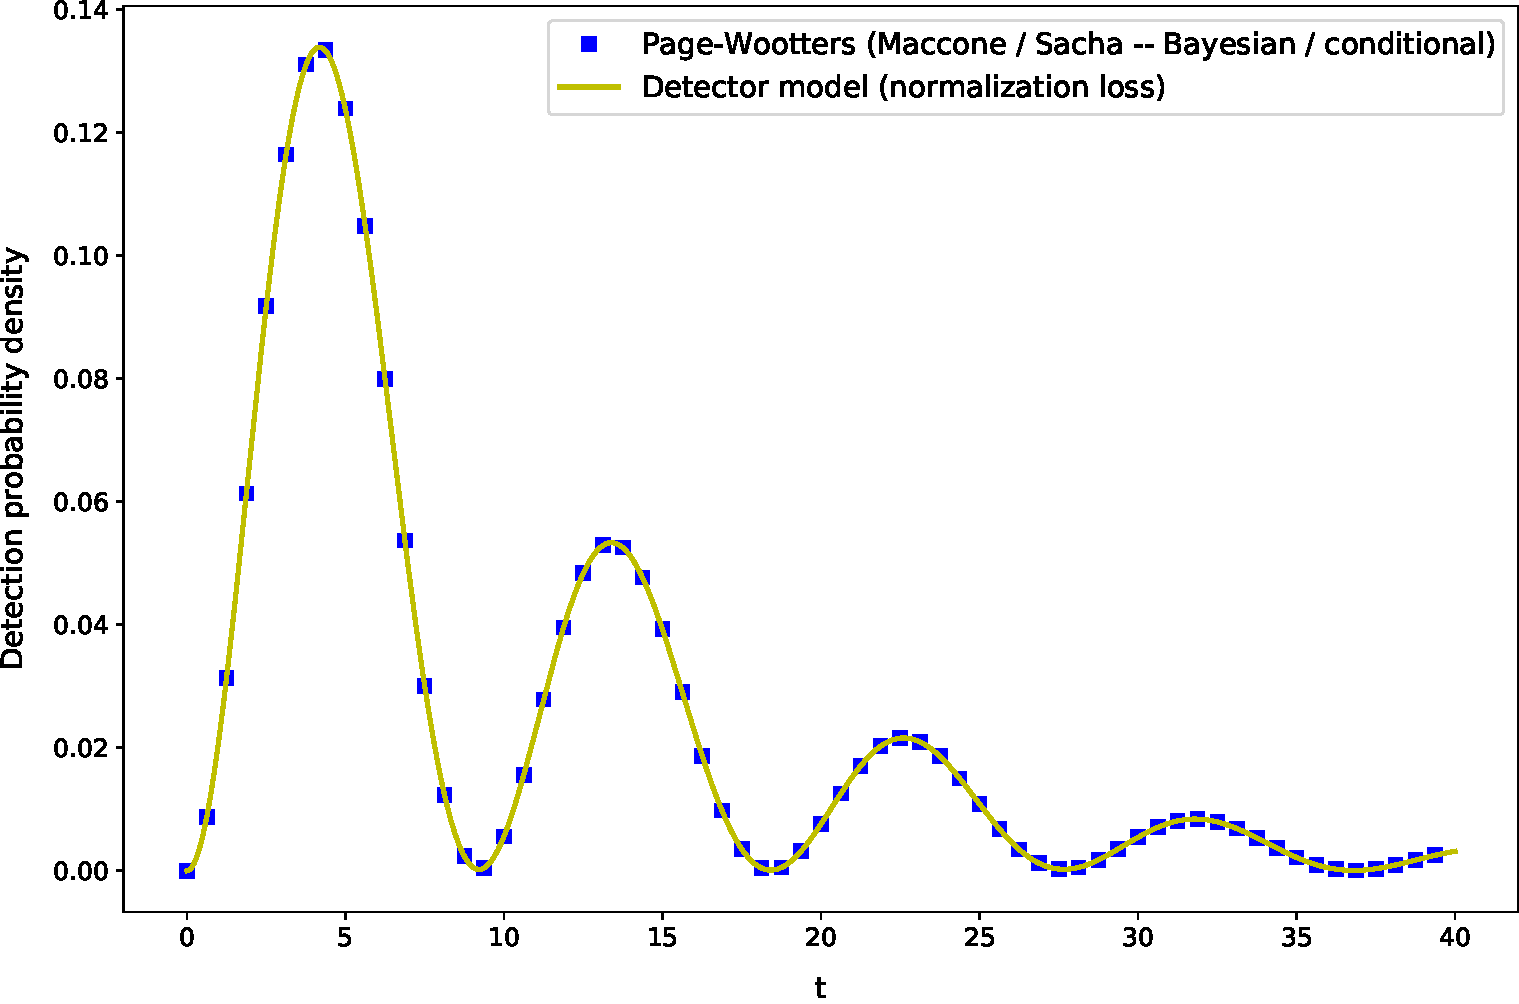
\includegraphics[width=\textwidth]{img/3ldetect/conditionalProbFit.pdf}
  \caption{Foo.}
  %\label{fig:psi_V}
\end{figure}